%%
% TUM Corporate Design LaTeX Templates
% Based on the templates from https://www.tum.de/cd
%
% Feel free to join development on
% https://gitlab.lrz.de/tum-templates/templates
% and/or to create an issue in case of trouble.
%
% tum-book class for lecture notes, Master's/Bachelor's thesis, ...
%
%%

\documentclass{tum-book}

\title{Analysis of Machine Learning for State Register Identification}
\author{Lee Seng Hwee}
\publisher{Bachelor of Science in Electrical Engineering and Information Technology}
\titledescription{Bachelor's Thesis\\
  \textbf{Bachelor of Science}\\
  Department of Electrical and Computer Engineering \\
  Technical University of Munich}
\fineprint{%
  \textbf{Supervised by}\\
  Prof.\ Dr.-Ing.\ Georg Sigl\\
  M.Sc.\ Johanna Baehr\\
  Chair of Security in Information Technology\\
  \vspace{12pt}
}
\usepackage{graphicx}
\usepackage[intoc,prefix]{nomencl}
\makenomenclature


\tolerance=1
\emergencystretch=\maxdimen
\hyphenpenalty=10000
\hbadness=10000

\begin{document}

\printthesisdisclaimer

\frontmatter

\cleardoublepage
\printnomenclature[3cm]

\nomenclature{$\rho_{phen}$}{Phenomenological term that represents scattering processes in the active region}
\nomenclature{$\hbar$}{Reduced Planck constant}

\tableofcontents

\mainmatter

\chapter{Introduction}
    \section{Hardware Vulnerability}\label{Hardware Vulnerability}
    In this fast-moving world, no one company can innovate and manufacture all minute components and modules itself. This is especially so in the designing and manufacturing of highly complex chips. Hence there is a strong reliance on third party solutions. With an increase in this reliance, there is an increase in opportunities for hardware security to be compromised, especially during the fabrication process, whereby additional backdoors can be implemented by the manufacturer. These backdoors which are not known to the designers can be exploited leading to loss of privacy, data and potentially system failures. In most cases this back-door can become hardware vulnerabilities which cannot be patched or takes time to be patched via a software update. Therefore, at those times, hardware might have to be replaced which can incur high amounts of cost and brand names associated with those hardwares, resulting in a detrimental decline of consumer trust.
    
    \section{Reverse Engineering Process}\label{Reverse Engineering Process}
    To mitigate the risk of hardware vulnerabilities caused by third party manufacturers, there is therefore a need to verify the manufactured chips especially if the manufacturer is not reputable. Hardware reverse engineering methods have been developed more in recent years to detect these security compromises, given the significant increase in complexity of chip designs. However traditional reverse engineering is still a tedious process as shown in Figure \ref{fig:Reverse Engineering Workflow}, involving depackaging, delayering, using of advanced imaging techniques to capture each layer and further processing to extract the netlist, which is explained in more detailed in paper\cite{baehr2020machine}. 
    
    \begin{figure}[ht]
        \centering
        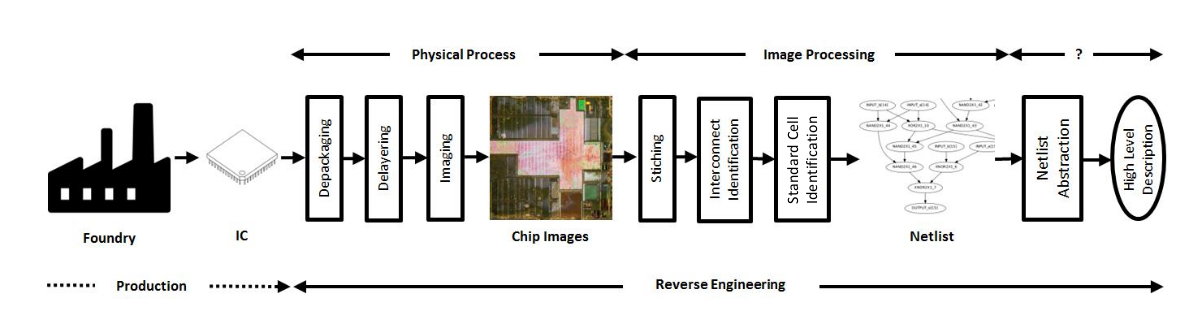
\includegraphics[scale=0.4]{myFiles/myImages/Reverse_Engineering_Process.png}
        \caption{Reverse Engineering Workflow\cite{baehr2020machine}}
        \label{fig:Reverse Engineering Workflow}
    \end{figure}
    
    
    \newpage\section{Severity of Hardware Vulnerability}\label{Severity of Hardware Vulnerability}
    To emphasize the severity of hardware vulnerability, past examples of hardware vulnerability, not specifically caused by manufacturers who added in back-door, can be used to elaborate this. "Meltdown"\cite{Lipp2018meltdown} and "Spectre"\cite{Kocher2018spectre} are 2 recent high profile cases of hardware vulnerabilities, which employed a similar form of attack on the processor, by targeting the isolation between the application and operating system and the isolation between applications respectively. This resulted in leakage of sensitive information. Luckily, these vulnerabilities could be patched via software patches.
    
    
    \section{Current Approaches}
    As explained in section \ref{Reverse Engineering Process}, reverse engineering is a tedious process, and this is especially true when dealing with State Register Identification from an extracted netlist. The current approach in identifying State Registers, requires designers with the full design information to compare the original design to reverse engineered design to identify if any additional gates or logic has been implemented. However, this method does possess limitations, commercial-of-the-shelf (COTS) ICs and SOCs with third-party IPs lack a golden model to be compared to.
    
    \subsection{RELIC and fastRELIC}\label{subsection:relic and fastrelic}
    To overcome the lack of a golden model, RELIC\cite{7527495} and fastRELIC\cite{8740844} were developed. RELIC and fastRELIC both use similar methods of finding potential state registers based on register pairs similarity scores (PSS). RELIC first pre-processes a gate level netlist to guarantee a similar gate structure, the State Registers from the netlist can be then separated out from the Data Registers, because the structure and functionality surrounding them is inherently different to the Data Registers, where the same functionality will happen more than once, i.e. for a 32 bit calculation, a function will occur 32 times. Comparing RELIC and fastRELIC, fastRELIC differs slightly by using a grouping mechanism, based on some parameters while RELIC chooses a specific parameter and declares any state registers with a lower cumulated PSS than that to be a State Register. This approach, though results high in accuracy, only rely on the PSS generated.
    
        \begin{figure}[h]
            \centering
            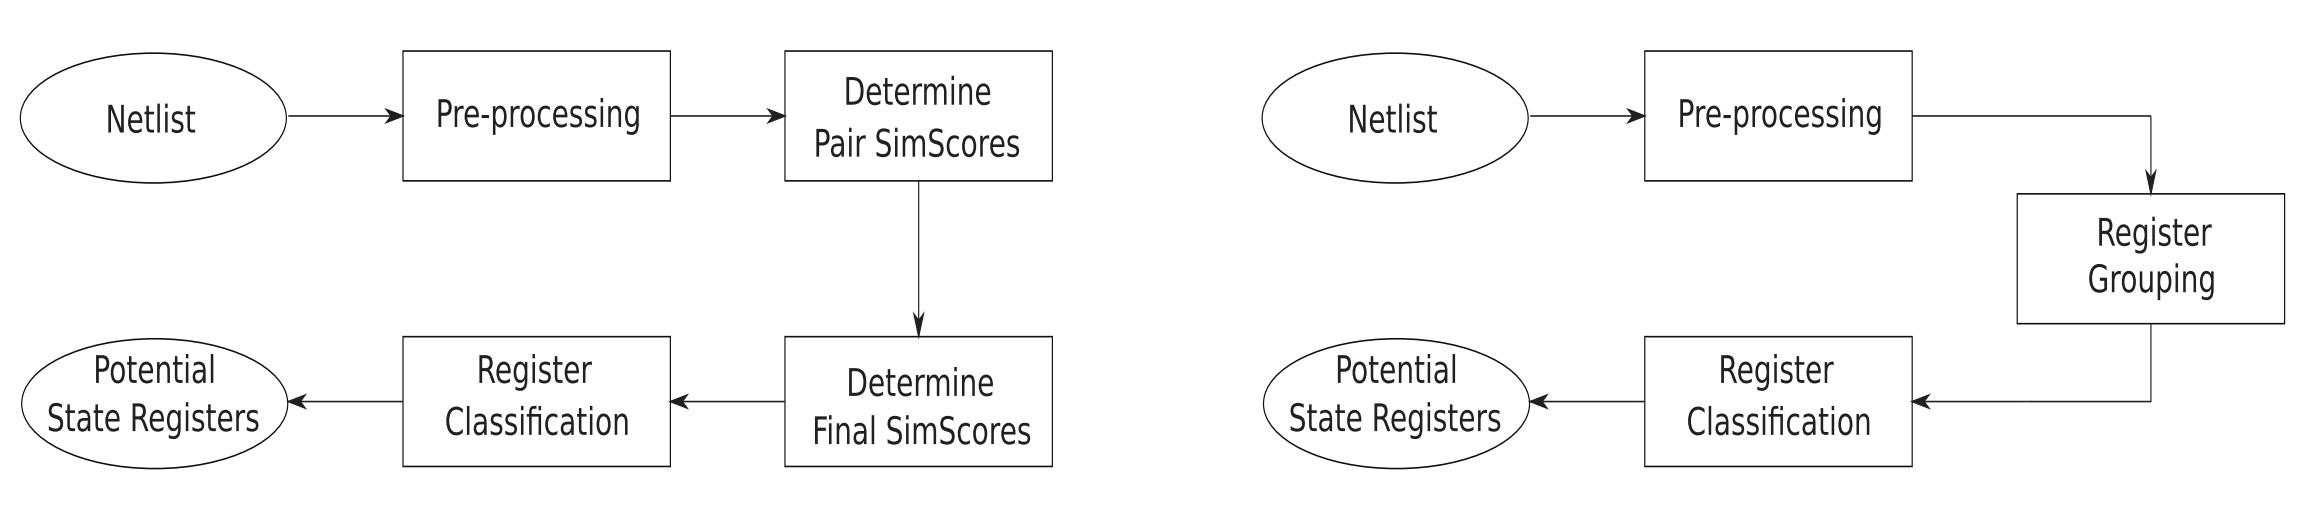
\includegraphics[scale=0.5]{myFiles/myImages/RELIC_and_fastRELIC.jpg}
            \caption{RELIC and fastRELIC}
            \label{fig:RELIC_and_fastRELIC}
        \end{figure}
        
    \bigskip\noindent
    The aim of this thesis is to train and deploy a neural network, using more features from the extracted netlist, aiding the decision making of classifying a Register into the categories of either 1 or 0 with 1 representing State Register and 0 representing non-State Register. 
    

\newpage\chapter{Pre-Processing}\label{chapter:pre-processing}
    \section{Features of Designs}\label{section:feature of design}
        Before the method of pre-processing is explained, the features and their meanings will be discussed. A register can be described in more than just the amount of difference between gates and flip-flops that makes it up. To further identify a register, features\cite{Schult08exploringnetwork} of the register and its neighbour can be used. In this section, the different types of features will be discussed. Before the discussion, some terminology can be explained as follows.
        
            \begin{itemize}
                \item Nodes: In a netlist can be represented by a gate or flip-flop with a specified depth. In this thesis, only the nodes represented by flip-flops are of interest.
                \item Depth of nodes: The number of steps between the last ancestor to be considered and the node. 
            \end{itemize}
    
        \bigskip\noindent
        For each register, a set of structural features were calculated, and these are discussed in the following subsections.
    
            \subsection{Average Neighbour Degree}
            Average Neighbour Degree is the average edges of a node in the neighborhood. It is also defined by the following expression.
                \begin{equation}
                k_{nn,i} = \frac{1}{|N(i)|} \sum_{j \in N(i)} k_j
                \end{equation}
            Where ${N(i)}$ are the neighbours of node $i$ and $k_j$ is the degree of node $j$ which belongs to $N(i)$
    
            \subsection{Betweenness Centrality}
            Betweenness centrality of a node $v$ is the sum of the fraction of all-pairs shortest paths that pass through $v$. It can be defined by using the expression
            
                \begin{equation}
                c_{B}(v) = \sum_{s,t \in V} \frac{\sigma(s,t |v)}{s,t}
                \end{equation}
                Where $V$ is the set of nodes, $\sigma(s, t)$ is the number of shortest $(s, t)-paths$, and $\sigma(s, t|v)$ is the number of those paths passing through some node $v$ other than $s, t$. If $s = t, \sigma(s, t) = 1$, and if $v \in {s, t}$, $\sigma(s, t|v) = 0$ 
    
            \subsection{Closeness Centrality}
            Closeness centrality $1$ of a node $u$ is the reciprocal of the average shortest path distance to $u$ over all $n-1$ reachable nodes.
                \begin{equation}
                C(u)=\frac{n-1}{\sum_{v=1}^{n-1} d(v,u)}
                \end{equation}
    
            \subsection{Clustering}
            For unweighted graphs, the clustering of a node u is the fraction of possible triangles through that node that exist,
                \begin{equation}
                c_u=\frac{2T(u)}{deg(u)(deg(u)-1)}
                \end{equation}
            where $T(u)$ is the number of triangles through nodes $u$ and $deg(u)$ is the degree of $u$.
    
            \subsection{Degree}
            The node degree is the number of edges adjacent to the node. The weighted node degree is the sum of the edge weights for edges incident to that node.
    
                \bigskip\noindent 
                This object provides an iterator for (node, degree) as well as lookup for the degree for a single node.
    
            \subsection{Degree Centrality}
            Defined as the number of links incident upon a node (i.e., the number of ties that a node has)\cite{Centrali48:online}
            
            \bigskip\noindent
            Let v* be the node with highest degree centrality in G. Let X:=(Y,Z) be the |Y|-node connected graph that maximizes the following quantity (with y* being the node with highest degree centrality in X):
            
                \begin{equation}
                    H=\sum _{{j=1}}^{{|Y|}}[C_{D}(y*)-C_{D}(y_{j})]
                \end{equation}
            \noindent    
            Correspondingly, the degree centralization of the graph G is as follows:
            
                \begin{equation}
                    C_{D}(G)={\frac {\sum _{i=1}^{|V|}[C_{D}(v*)-C_{D}(v_{i})]}{H}}
                \end{equation}

            \noindent
            The value of H is maximized when the graph X contains one central node to which all other nodes are connected (a star graph), and in this case
            
                \begin{equation}
                    H=(n-1)\cdot ((n-1)-1)=n^{2}-3n+2.
                \end{equation}
            
            \noindent
            So, for any graph G:=(V,E)
            
                \begin{equation}
                    C_{D}(G)={\frac {\sum _{i=1}^{|V|}[C_{D}(v*)-C_{D}(v_{i})]}{|V|^{2}-3|V|+2}}
                \end{equation}

            
            \subsection{Indegree}
            The node in-degree is the number of edges pointing in to the node.
            
            \subsection{Has Feedback Path}
            A node has a feedback path if there exists a loop from the output of the node to its input.
    
            \subsection{Katz}
            Katz centrality computes the centrality for a node based on the centrality of its neighbors. It is a generalization of the eigenvector centrality. The Katz centrality for node i is
                \begin{equation}
                x_i=\alpha\sum_{j}A_{ij}x_j+\beta
                \end{equation}
            
                \bigskip\noindent where $A$ is the adjacency matrix of graph $G$ with eigenvalues $\lambda$.The parameter $\beta$ controls the initial centrality and
            
                \begin{equation}
                \alpha<\frac{1}{\lambda_{max}}
                \end{equation}
    
            \subsection{Load Centrality}
            The load centrality of a node is the fraction of all shortest paths that pass through that node.
    
            \subsection{Outdegree}
            The node out-degree is the number of edges pointing out of the node.
    
            \subsection{Pagerank}
            PageRank computes a ranking of the nodes in the graph G based on the structure of the incoming links. It was originally designed as an algorithm to rank web pages.
    
            \subsection{xx good SN}
            This feature indicates a good starting node for RELIC/fastRELIC search algorithms. Hence it is not useful in this machine learning use case and therefore will be dropped prior to any feature selections method.
            
            \subsection{xx state ff}
            This feature will represent if a register is or is not a state register by assigning $1$ or $0$ respectively. The goal of the neural network model is to be able to input any arbitrary registers and predict whether the register is or is not a state register, by assigning it a $1$ or $0$.




    \newpage\section{Pre-Processing for Artificial Neural Network}\label{section:pre-processing for artificial neural network}
        \subsection{Scaling}\label{subsection: scaling}
        Before creating a neural network to train and predict the classification of the registers, a given data set containing the features mentioned in section \ref{section:feature of design} with different number of flip-flops in each file, has to be pre-processed. First the targeted feature in this case "xx state ff" has to be identified and removed from the files followed by scaling down of the data set to values between 0 and 1, using the module "Scikit learn"\cite{scikit-learn} as the values of some features ranges between 0 to 1 while others between 0 to 10, eg, outdegree has a range between 2 to 5, clustering has a range between 0 to 0.1. Due the difference in ranges for each feature, scaling is necessary to ensure that there is no biasness from the neural network due to one feature having higher values than the other.
 
        \subsection{Methodology of additional features}\label{subsection:methodology of additional features}
        5 different implementations of the given data sets listed were chosen to train the neural network.
        \bigskip\begin{itemize}
            \item Original features present in the data set 
            \item Original features present in the data set with fastRELIC(PSS) as an additional feature
            \item Original features present in the data set with Cosine Similarity as an additional feature
            \item Original features present in the data set with Euclidean distance as an additional feature
            \item Original features present in the data set with Euclidean and fastRELIC as additional features
        \end{itemize}
        The additional features are scaled using the same method as the other features. Results of each run will be further discussed in Chapter \ref{chapter:results}.
        
        
        \subsubsection{Original Features}
        Previous works have already calculated a set of features for the data set, which can be found in section \ref{section:feature of design}, these features will be known as Original features.

        \newpage\subsubsection{fastRELIC}\label{subsubsection:pss}
        To use the fastRELIC method as an additional feature, the PSS is used. A PSS between 0 to 1 is produced for the pair register and the values produced are influenced by the selected depth of the design in the algorithm. A threshold of $0.7$ selected in the experiments and a counting algorithm is used to count the similarity score of a register to other registers above the threshold. These counts are then normalized as not all data sets have the same number of registers. The number of similarity counts can be interpreted by the higher the count, the more registers the targeted register is similar to, therefore, the lower the count, the higher the probability that the register is a State Register. 

        \bigskip\subsubsection{Cosine Similarity}\label{subsubsection:cosine similarity}
        The cosine similarity is a measurement of cosine angle between 2 non-zero vectors. The result from this measurement determines how similar the 2 vectors are, in the direction they are pointing to. The mathematical expression of cosine similarity can be determined by the manipulation of the inner product mathematical equation.

            \bigskip\noindent The inner product of 2 $n^{th}$-dimensional vectors $u$ and $v$ is defined as:
            \begin{equation}
                \label{eqn:dot product}
                u\cdot v = |u||v|cos(\theta)
            \end{equation}
            \noindent 
            Where $\theta$ is the angle between $u$ and $v$, therefore the cosine similarity is given to be:
            \begin{equation}
                \label{eqn:cosine similarity}
                cos_{sim}(u,v)=cos(\theta)=\frac{u\cdot v}{|u||v|} 
            \end{equation}
            
            \noindent 
            To use cosine similarity as a feature, first the register's shape shown in Figure \ref{fig:Register Shape} is extracted by selecting a depth. The register's shape is expressed as a vector with each dimension representing the number of same gates or flipflops the register has, shown in Figure \ref{fig:vector}. In this example, the 2 that is boxed in Figure \ref{fig:vector} corresponds to the two inverters boxed in Figure \ref{fig:Register Shape}. After calculating the cosine similarity, similar to how PSS is implemented, a threshold is selected, and a counting algorithm is used to count the number of registers each register is similar to. Only a similarity score of more than then the selected threshold will be counted by the counting algorithm. The result is then normalized to ensure fairness.The lower the count, the higher the probability that the register is a State Register. 
            

            \begin{figure}[h]
                \centering
                \begin{minipage}[b]{0.35\textwidth}
                    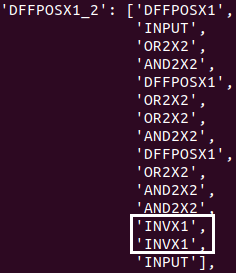
\includegraphics[width=\textwidth]{myFiles/myImages/shape_vector_1.png}
                    \caption{Register shape}
                    \label{fig:Register Shape}
                \end{minipage}
                \hfill
                \begin{minipage}[b]{0.35\textwidth}
                    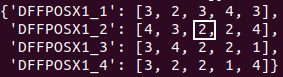
\includegraphics[width=\textwidth]{myFiles/myImages/vector.png}
                    \caption{vector}
                    \label{fig:vector}
                \end{minipage}
            \end{figure}

            \newpage\noindent
            However, this method is not implemented in the final testing. As from initial testing, the count value for the method of cosine distance does not differ significantly between any two registers, only by $<10\%$. This resulted in a similar count score, for all registers, depending on the selected threshold, which was selected to be $0.9$. This led to poorer performance at times when compared to the original files initial testings. Refer to Section \ref{subsection:implementing additional features} for testing methodology.

        \subsubsection{Euclidean Distance}\label{subsubsection:euclidean distance}
        The euclidean distance of 2 vectors is the measurement of the shortest distance between 2 points of the vector. The closer they are, the larger the similarity. In Figure \ref{fig:Euclidean Distance}, the euclidean distance between 2, 2-dimensional vectors, $u$ and $v$ is represented by $d$.
    
            \begin{figure}[h]
                \centering
                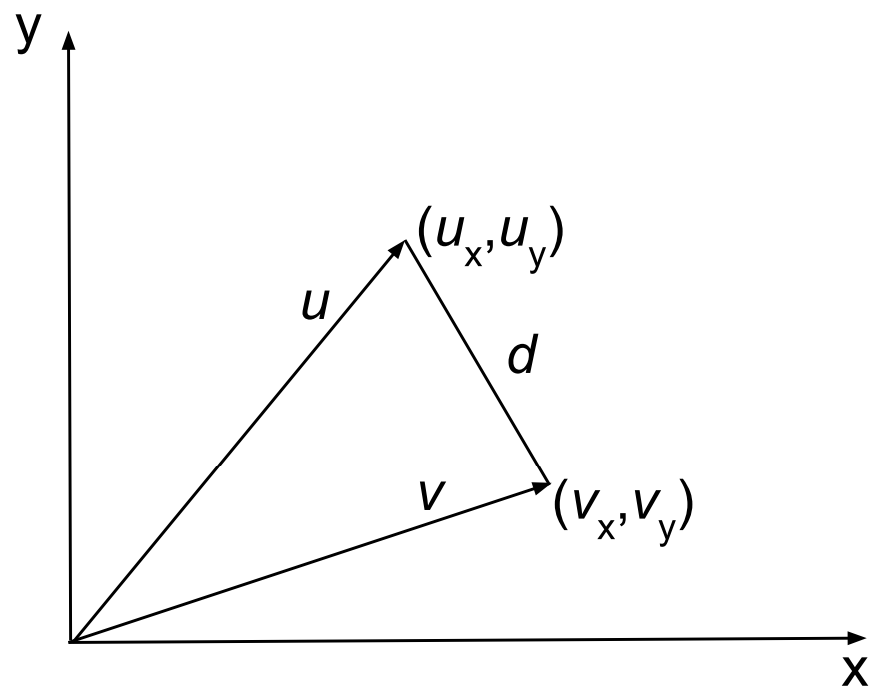
\includegraphics[scale=0.75]{myFiles/myImages/Euclidean_Distance.png}
                \caption{Euclidean Distance}
                \label{fig:Euclidean Distance}
            \end{figure}
    
            \bigskip\noindent
            The distance $d$ can be calculated by 
            \begin{equation}
                \label{eqn:euclidean distance}
                E(u, v)=\sqrt{(u_x - v_x)^2+(u_y-v_y)^2}
            \end{equation}
            \noindent
            In a $n^{th}$-dimensional vector, it can be represented by
            \begin{equation}
                \label{eqn:euclidean distance nth dimension}
            E(u, v)=\sqrt{\sum_{i=1}^{n} {(u_{i} - v_{i})^2}}
            \end{equation}
    
            \bigskip\noindent
            Following the extraction method for the register shape, which is then expressed as a vector detailed in Section \ref{subsubsection:cosine similarity}, the euclidean distance between the any 2 register's vector can be calculated using Equation \ref{eqn:euclidean distance nth dimension}. A threshold of $2.4$ is then selected for the experiments and a counting algorithm is used. The count is incremented if the euclidean distance is below the selected threshold, as this implies the compared vectors are close and thus similar. The lower the count, the higher the probability that the register is a State Register.

        \newpage\subsection{Feature Selection}\label{subsection:features selection}
        Feature selection has been shown to be one of the most important steps before implementing the model as it will severely impact the training of the model. The benefits of doing feature selection is listed as follows\cite{feature_selection}.
        
            \begin{itemize}
                \item Reduces Overfitting: Less redundant data, lesser the opportunity for the network to be influenced by these features 
                \item Improves Accuracy: Less misleading data improves model accuracy as the neural network does not have to take into account the patterns of these features
                \item Reduces Training Time: Less data points reduce algorithm complexity resulting in reduced time taken to train the model
            \end{itemize}
            
            \bigskip\noindent 
            Due to the clear advantages of performing feature selection, five methods of feature selection were performed.
            \begin{itemize}
                \item Constant Filtering
                \item Quasi-Constants Filtering
                \item Feature Permutation
                \item Sequential Feature Selection 
            \end{itemize}

        \subsubsection{Constants Filtering}\label{subsubsection:constant filtering}
        Constants Filtering was first decided as is computationally inexpensive yet provides a simple and fast approach. This method was based on the concept that constant values in a feature, does not add any value to the neural network as it does not present a pattern to the neural network. Hence removing such features will reduce the training time of the neural network. This was done via the module "scikit-learn" for python.
        
        \subsubsection{Quasi-Constants Filtering}\label{subsubsection:quasi-constant filtering}
        Based on similar reasoning in using constants filtering, quasi-constant filtering method differs from constant filtering by adding a threshold. If the difference between any 2 features is not more than a selected threshold in percentage, the feature will be removed.
        
        \subsubsection{Feature Permutation}\label{subsubsection:feature permutation}
        Feature Permutation is based on the concept whereby permuting the values in a feature breaks the relations between the permuted feature and the rest of the features. This loss of relation should decrease the accuracy significantly (more than a selected threshold) if the feature is important and increase/remain constant if the feature has no impact or hinders the neural network. To determine if a feature is important, the two methods of testing the feature importance is detailed in Section \ref{section:feature permutation results}. Each feature in the data set is permuted individually, fitted, and tested on a neural network for $k$ runs. The average accuracy after $k$ runs for each feature is recorded and compared individually to the unpermuted feature set average accuracy after $k$ runs.The feature will be removed if the accuracy is the same, or when the difference is below the selected threshold. The flow of the process can be seen in Figure \ref{fig:Feature Permutation Flow Chart}.
        
        \newpage
        \begin{figure}[ht]
            \centering
            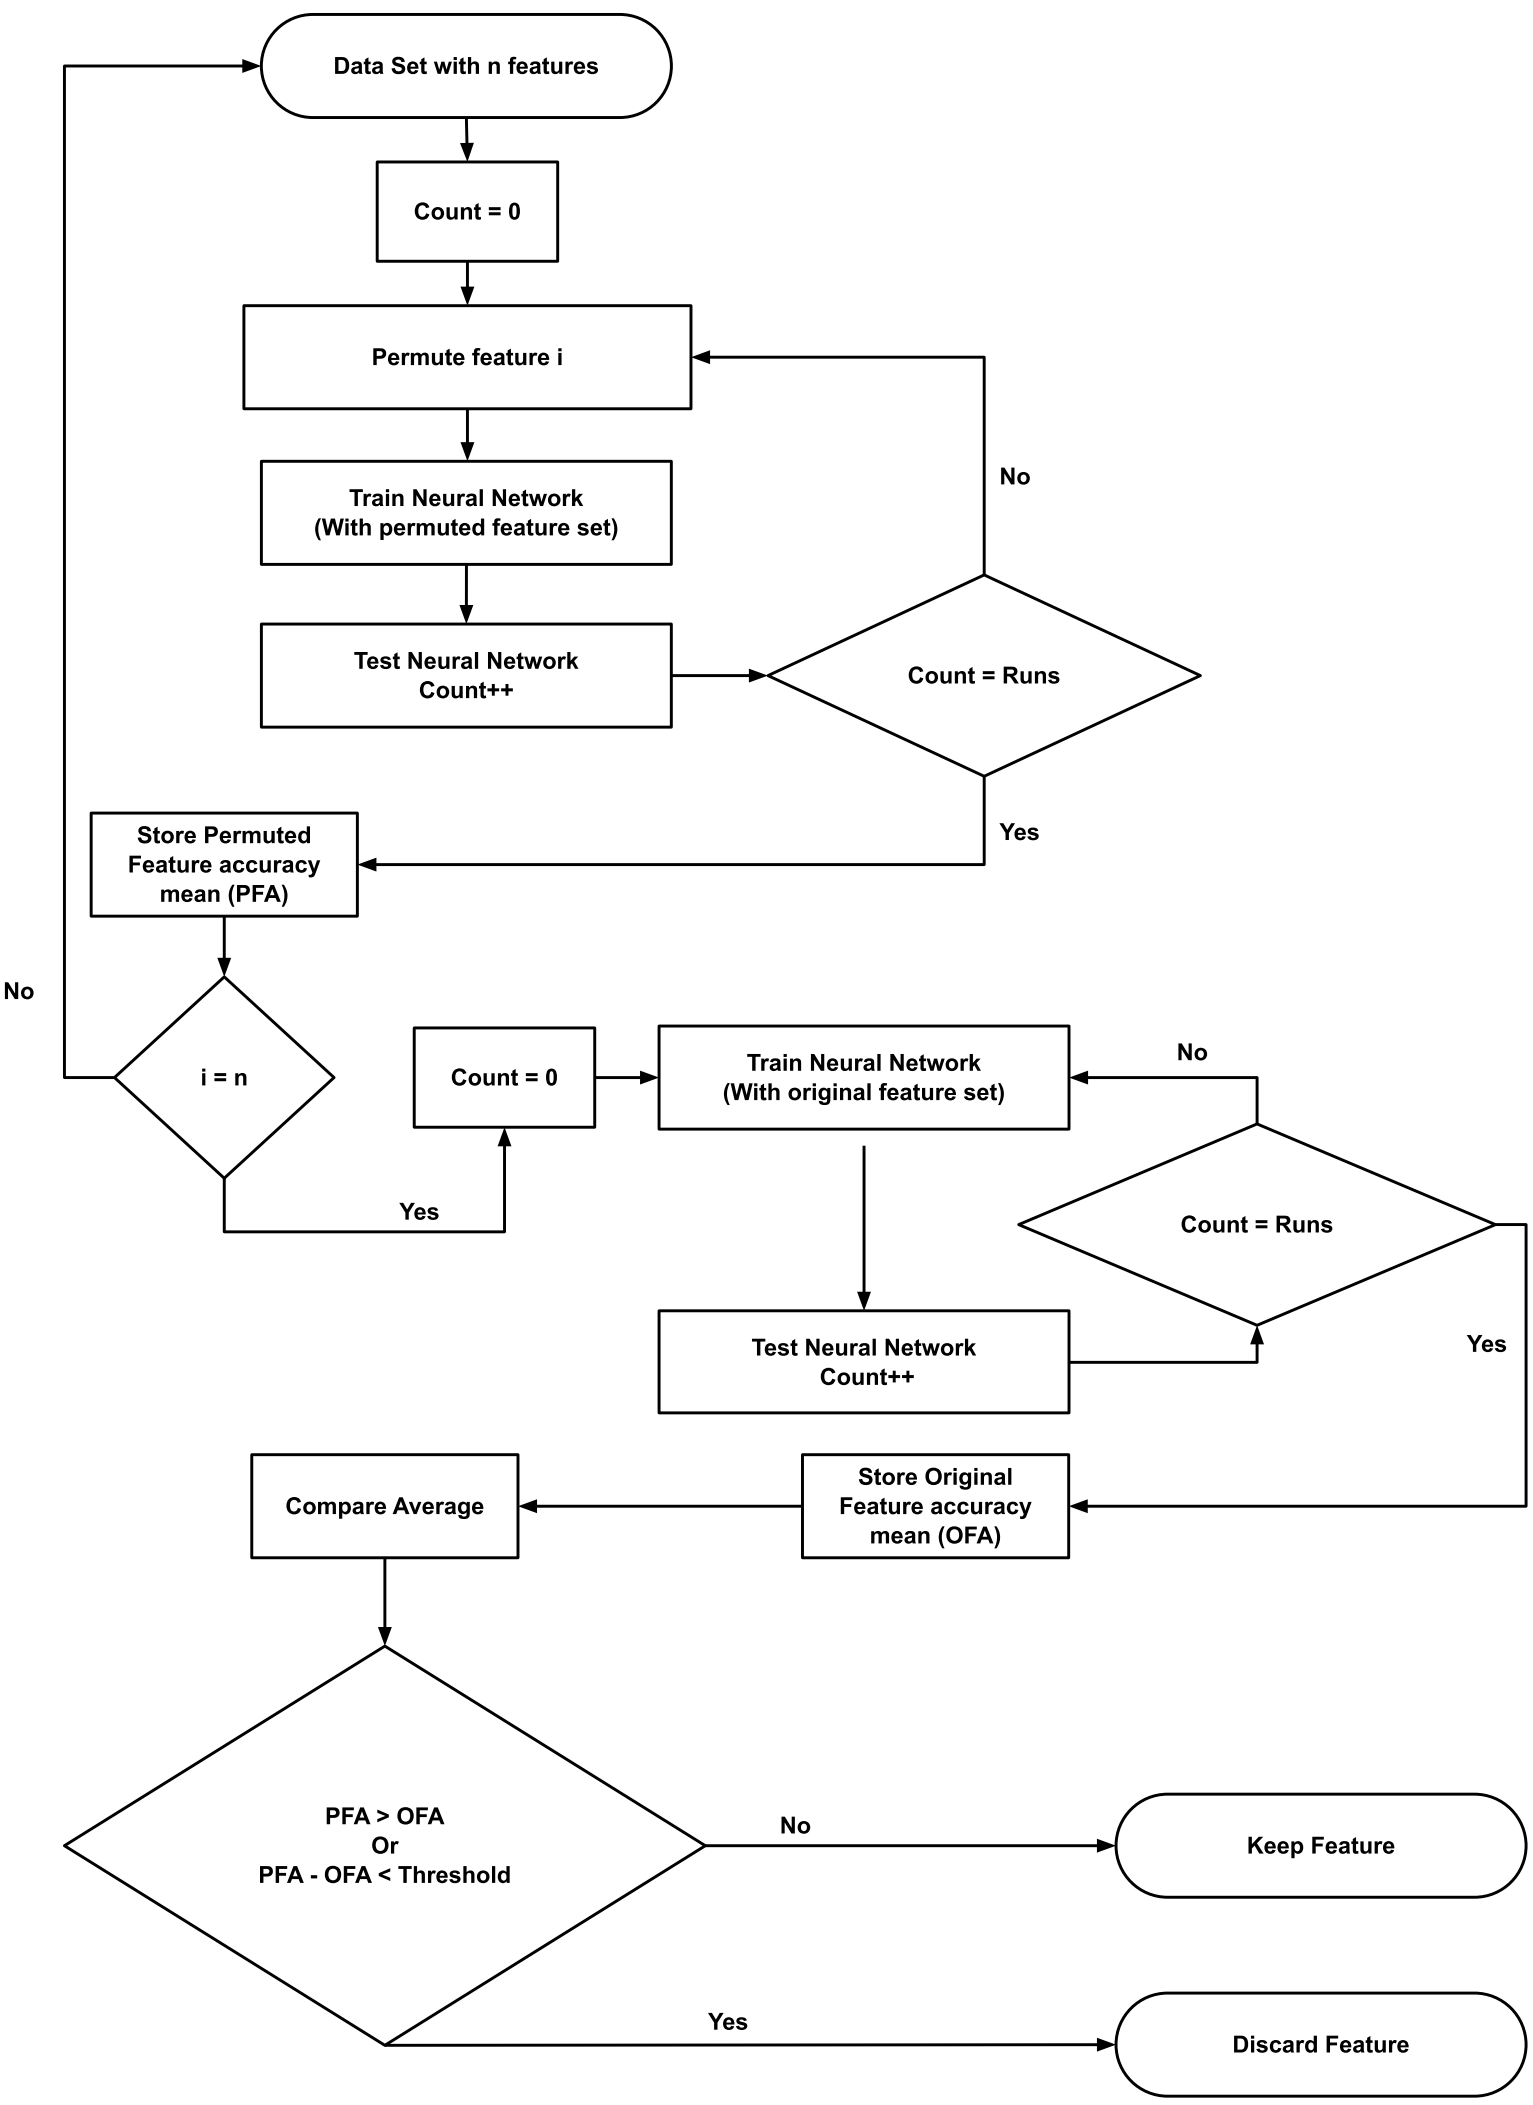
\includegraphics[scale=0.5]{myFiles/myImages/Feature_Permutation.png}
            \caption{Feature Permutation Flow Chart}
            \label{fig:Feature Permutation Flow Chart}
        \end{figure}
        
        \bigskip\noindent
        In Figure \ref{fig:Feature Permutation Flow Chart}, the data set is fed to the neural network and a counter is initialized to 0. The first of the $n$-features is permuted and trained on the neural network. An accuracy is produced by testing the neural network and this process is repeated for a selected number of runs (runs = 100 for the experiments). Once the counter equals to the number of selected runs, an average accuracy will be calculated and the next feature is selected. This process is repeated for all features. Next the unpermuted data set is trained and tested on the neural network for the same number of runs and an average accuracy is calculated. The average permuted accuracy of each feature is compared to the unpermuted average accuracy and the feature will then be discarded or retained based on the set of conditions.
        
        
        \newpage\subsubsection{Sequential Feature Selection}\label{subsubsection:Sequential Feature Selection}
        Sequential Feature Selection selects the best features combination of feature set, based on a recursive combinations testing. To implement Sequential Feature Selection, a module "mlxtend"\cite{raschkas_2018_mlxtend} was chosen. First the algorithm evaluates the neural network performance on each feature and the highest performing feature is selected. Next the selected feature will be in a combination two with all other features and the performance of the neural network is evaluated again. This process will then be carried out until the desired number of features is reached.
        
            \bigskip\begin{figure}[h]
                \centering
                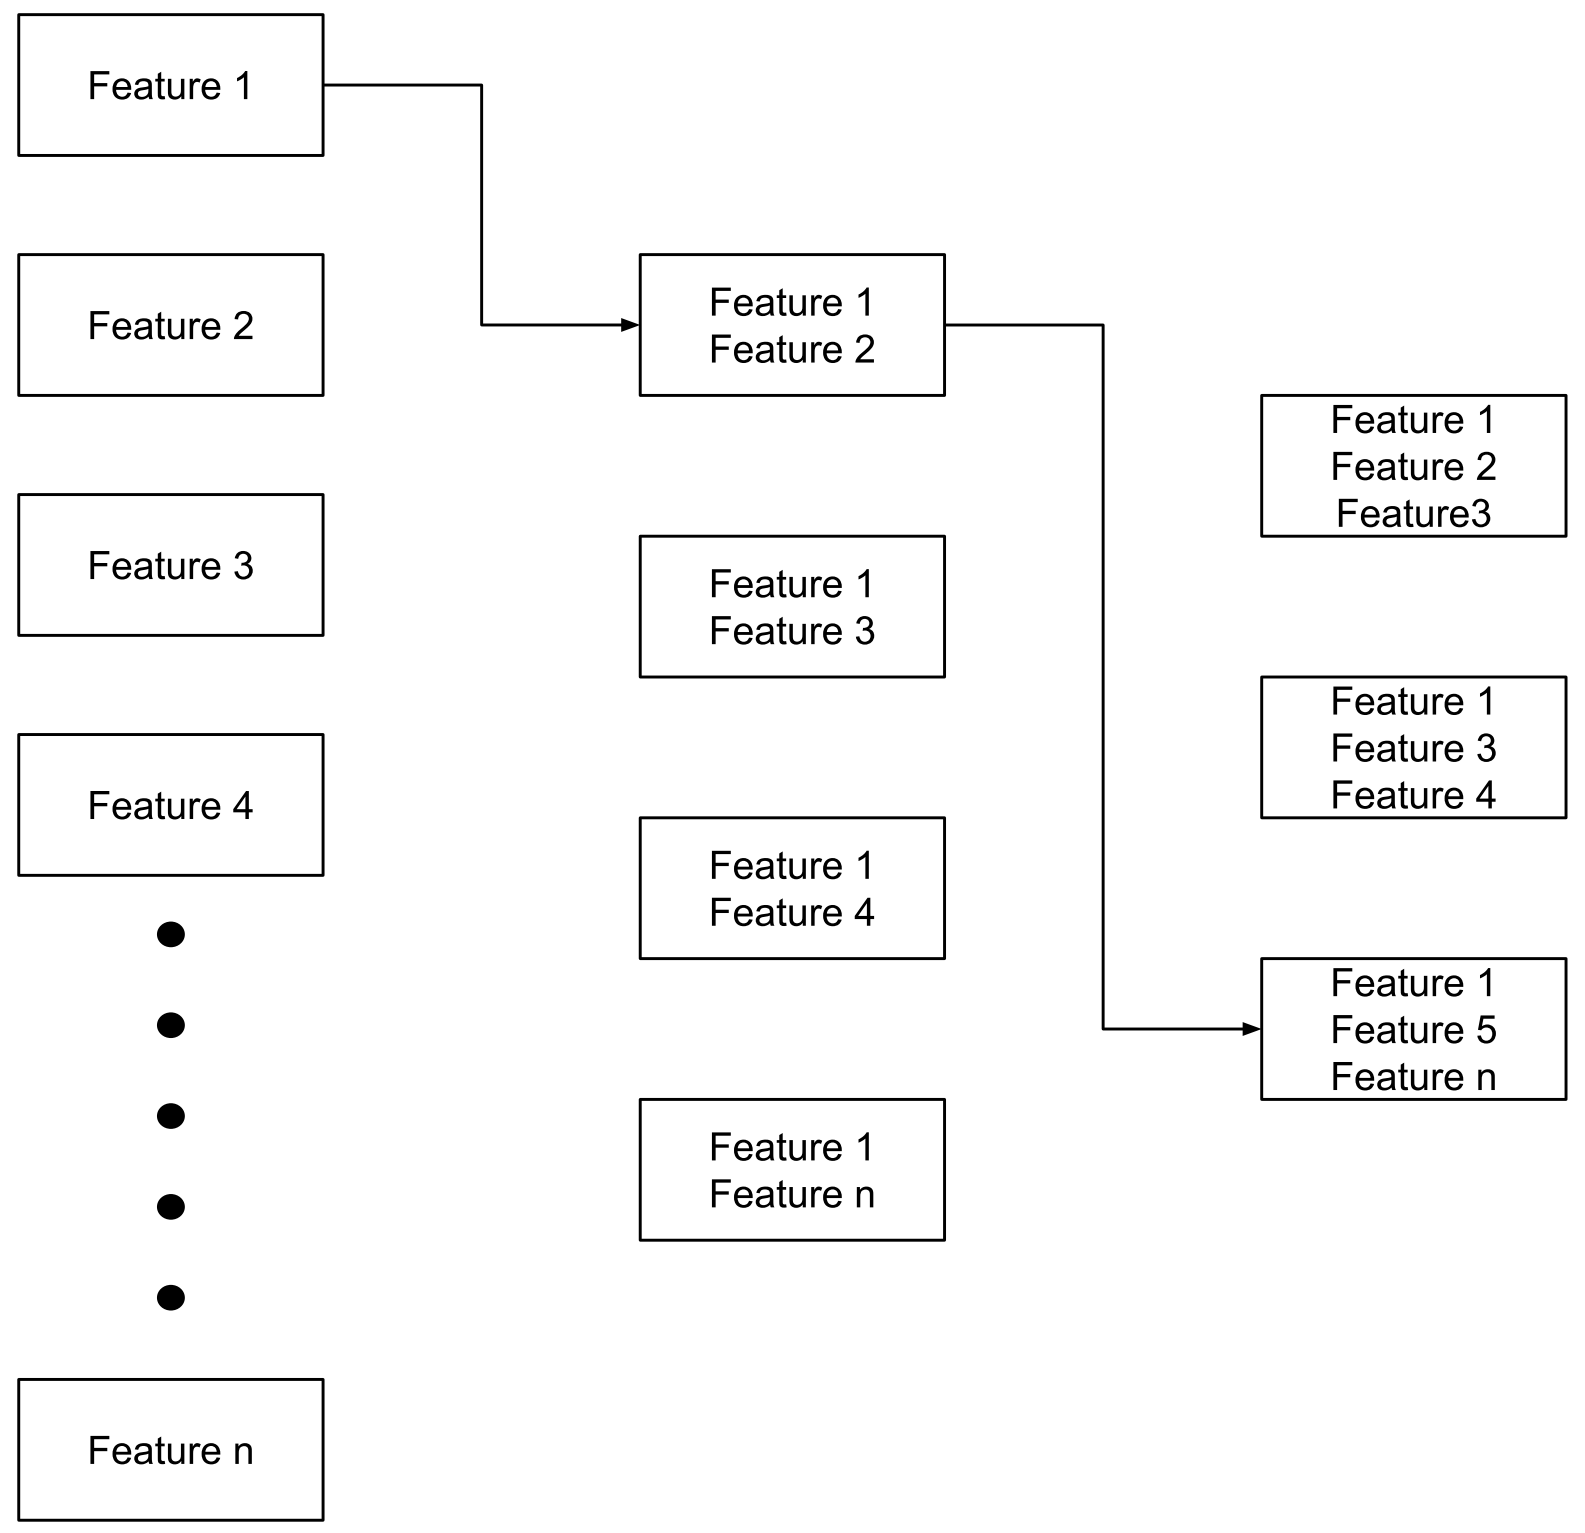
\includegraphics[scale=0.5]{myFiles/myImages/Sequential_Feature_Selection.png}
                \caption{Sequential Feature Selection Flow Chart}
                \label{fig:Sequential Feature Selection Flow Chart}
            \end{figure}
        
        \noindent
        In Figure \ref{fig:Sequential Feature Selection Flow Chart}, Sequential Feature Selection is performed on a data set with $n$-features. Evaluation is done individually for all features and the feature with the highest accuracy is chosen, which is feature 1 in Figure \ref{fig:Sequential Feature Selection Flow Chart}. A combination of two, containing feature 1 and one other feature is evaluated again, selecting the combination with the highest accuracy. This process is continued until the selected amount of feature provided by the user is reached. In the experiments for this thesis, the upper limit of the number of features is selected to be all features after the filtering method. Based on the results in Section \ref{subsection:Sequential Feature Selection result}, the average number of features selected from the data set lies between 8 to all features after implementing this feature selection method.
    



\chapter{Neural Network Model}\label{chapter:neural network model}
    \section{Understanding the Neural Network}\label{section:understanding the neural network}
    Machine Learning\cite{Learnhow39:online} uses data to train a model which can be then used to identify patterns and predict a future set of values. Machine learning can generally be classified into 2 types, supervised and unsupervised. In supervised machine learning problems, the problems can then be further classified into 2 different types of problems, regression, and classification. In regression machine learning problems, the model’s predicted outcomes using the trained data are typically real numbers, while classification machine learning data outcomes are usually classes or categories of which the data belongs to. In unsupervised machine learning, a data set is passed and by applying different algorithms and statistical data, the goal of an unsupervised machine learning model is to get the model to identify the structure of the given data set.

        \bigskip\noindent
        The model used to classify if a register is or is not a state register will be a supervised machine learning model. Machine learning is generally only a single layer, using an estimator (classification or regression) to perform predictions and requires humans to input the best feature to learn from. Deep learning, a subset of machine learning on the other hand uses multiple layers by connecting neurons between layers, interacting directly with the data set to learn what are the most important features. Deep learning uses the neural network to perform prediction and an optimizer to back propagate to adjust the weights and bias for better predictions. Figure \ref{fig:Single Neuron Neural Network} shows a single neuron neural network with multiple different hyperparameters such as activation function, threshold and transfer functions, these hyperparameters will be further explained in details in Section \ref{section:hyperparameters}. By adding more layers and neurons, the neural network is then known as a multilayer perceptron neural network. The general diagram for a multilayer perceptron neural network can be seen in Figure \ref{fig:Deep Feed Forward Neural Network}.

        \bigskip\begin{figure}[h]
            \centering
            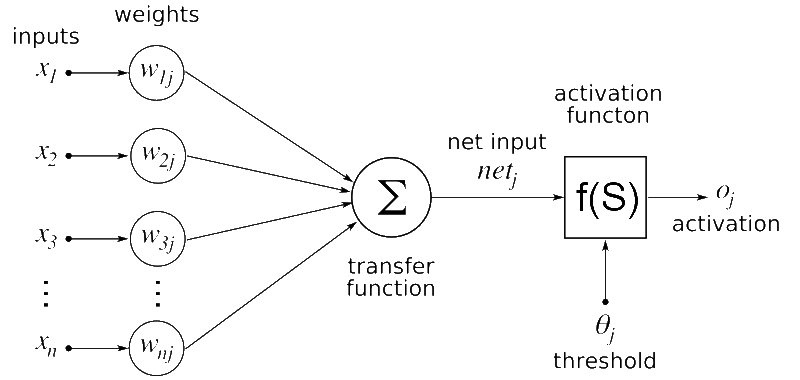
\includegraphics[scale=0.5]{myFiles/myImages/Artificial_neural_network.png}
            \caption{Single Neuron Neural Network\cite{SingleNeuron}}
            \label{fig:Single Neuron Neural Network}
        \end{figure}

        \bigskip\noindent
        The mathematical expression of a single neuron neural network is given to be:
        \begin{equation}
        \label{eqn:n layers neural network}
        f(S)=f(b + \sum_{i=1}^{n} x_iw_i)
        \end{equation}
        
        \noindent
        which is based on the equation of a straight line. 

        \newpage\noindent
        There are multiple different architectures for a neural network, such as Deep Feed Forward Neural Network (FNN), Convolution Neural Network(CNN), Recurrent Neural Networks(RNN) and many others, each having their own unique designs, suited for different purposes. Due to the nature of this thesis, of using Directed Graphs, the architecture of FNN is selected. To create this neural network, layers of densely connected neurons are stacked together. This is depicted in Figure \ref{fig:Deep Feed Forward Neural Network}
        
        \bigskip\begin{figure}[h]
            \centering
            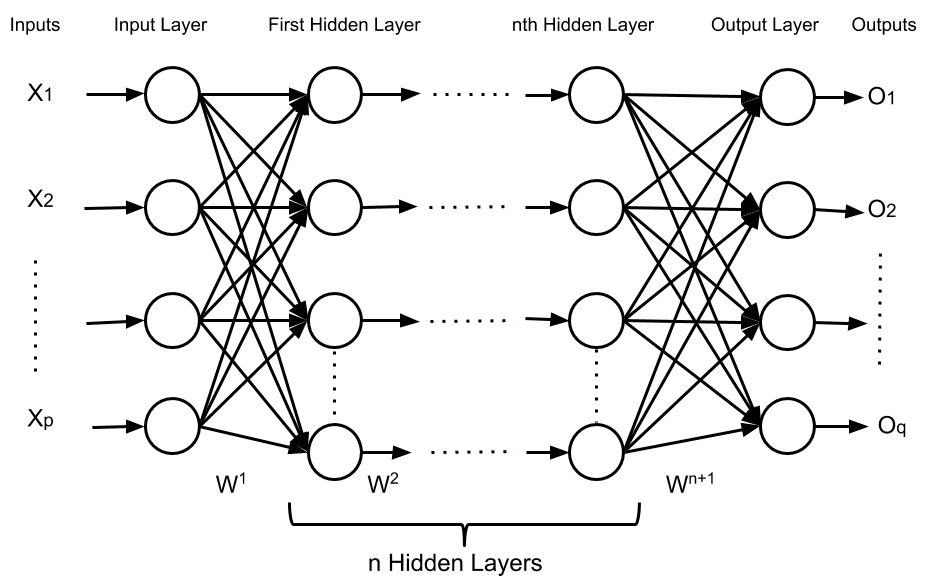
\includegraphics[scale=0.5]{myFiles/myImages/FNN.png}
            \caption{Deep Feed Forward Neural Network\cite{DeepFeedForwardNeuralNetwork}}
            \label{fig:Deep Feed Forward Neural Network}
        \end{figure}
        
        \bigskip\noindent
        The question of how many layers there should be or what is the most suitable layer for the data set the neural network is training on arises. The most suitable amount of layer cannot be stated as easily as it depends on the complexity of the data set. In general, the more layers there are, the higher the abstract representation of the input the neural network can build. However, this does not mean that the more the layers, the better the trained model will be. If a data set is of low complexity and is fed through a neural network of high layers, there is a very high chance of overfitting the model. Thus, this is a parameter to consider when training the neural network.

    \newpage\section{Hyperparameters}\label{section:hyperparameters}
    Aside from deciding on the number of layers in the neural network, there are multiple other parameters known as hyperparameters in a neural network to tune. In this section the various hyperparameters and how they affect the neural network will be discussed.

        \subsection{Activation function}
        As shown in Figure \ref{fig:Single Neuron Neural Network}, there is a function $f(s)$ represented as $f(x)$ in the following explanation of the different types of activation functions. The role of the activation function is to map the output of a single neuron to a more suited value, adding non-linearity to the model. There are multiple different activation functions, however only the most used activation function will be discussed. 
        
            \bigskip\noindent 
            Types of activation function:
            \begin{itemize}
                \item Sigmod
                \item ReLU
                \item ELU
                \item tanh
            \end{itemize}

        \subsubsection{Sigmod}
        The sigmoid function maps the output of the neuron to a value between $0$ and $1$. This function is particularly useful in a binary situation, e.g. (true or false), (yes or no), (1 or 0). However the function does have a vanish gradient problem as shown in the derivative of the function in Figure \ref{fig:Sigmoid Function}. 
        
            \begin{figure}[h]
                \centering
                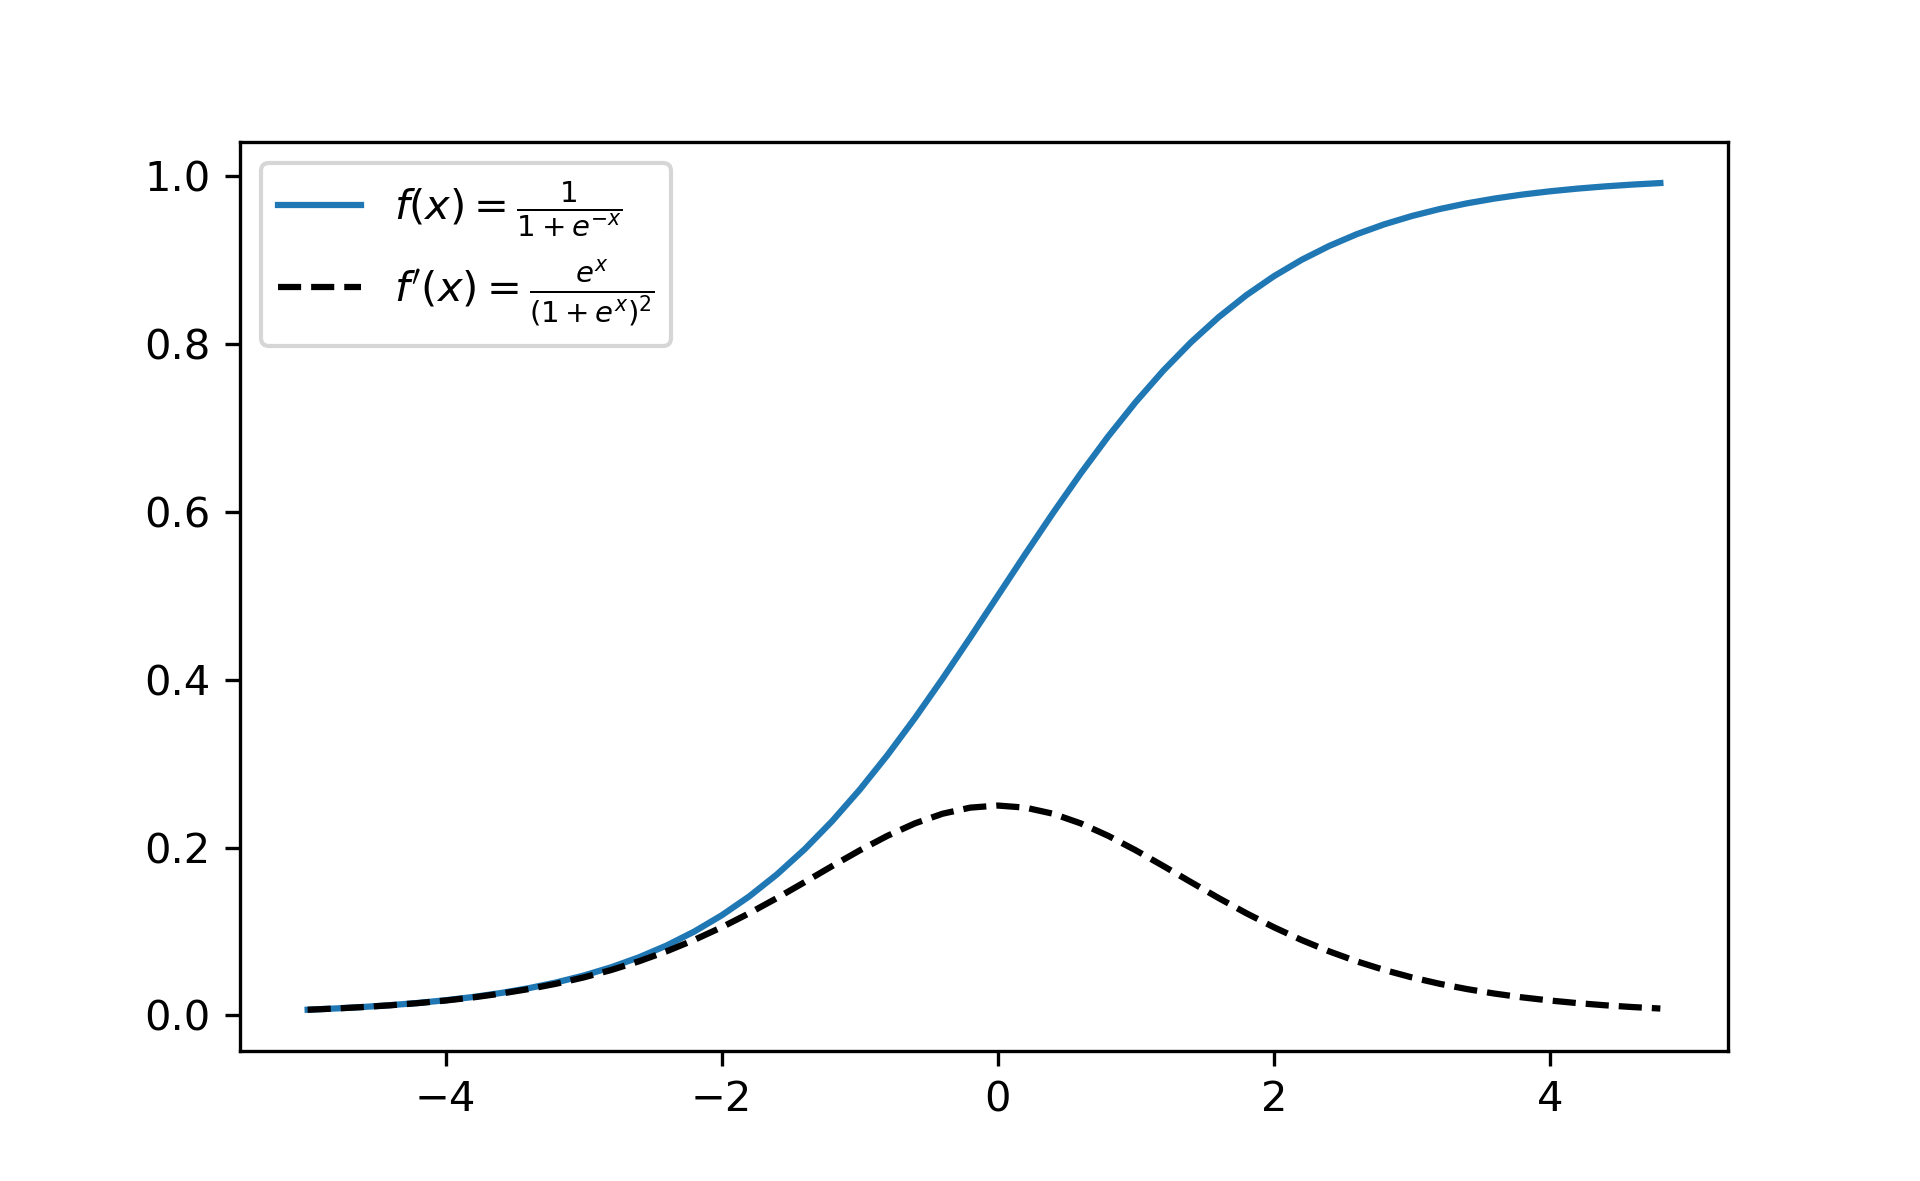
\includegraphics[scale=0.75]{myFiles/myImages/Sigmoid.png}
                \caption{Sigmoid Graph}
                \label{fig:Sigmoid Function}
            \end{figure}
            
        \noindent
        Vanishing gradient problems occur when more layers using certain activation functions are added. This will then cause the gradient of loss function to approach 0, making the training of the neural network harder.

            \newpage\subsubsection{ReLU}
            ReLU is the most common activation function in a neural network as it returns the input value when the input is more than 0 and 0 if the input is less than 0. ReLU can be used especially when the designer of the neural network is unsure of what activation function to use. ReLU also comes with its benefits of being non-computationally intensive and due to its linearity, does not have the vanishing gradient problem as shown in Figure \ref{fig:ReLU Function}.
            
                \begin{figure}[h]
                    \centering
                    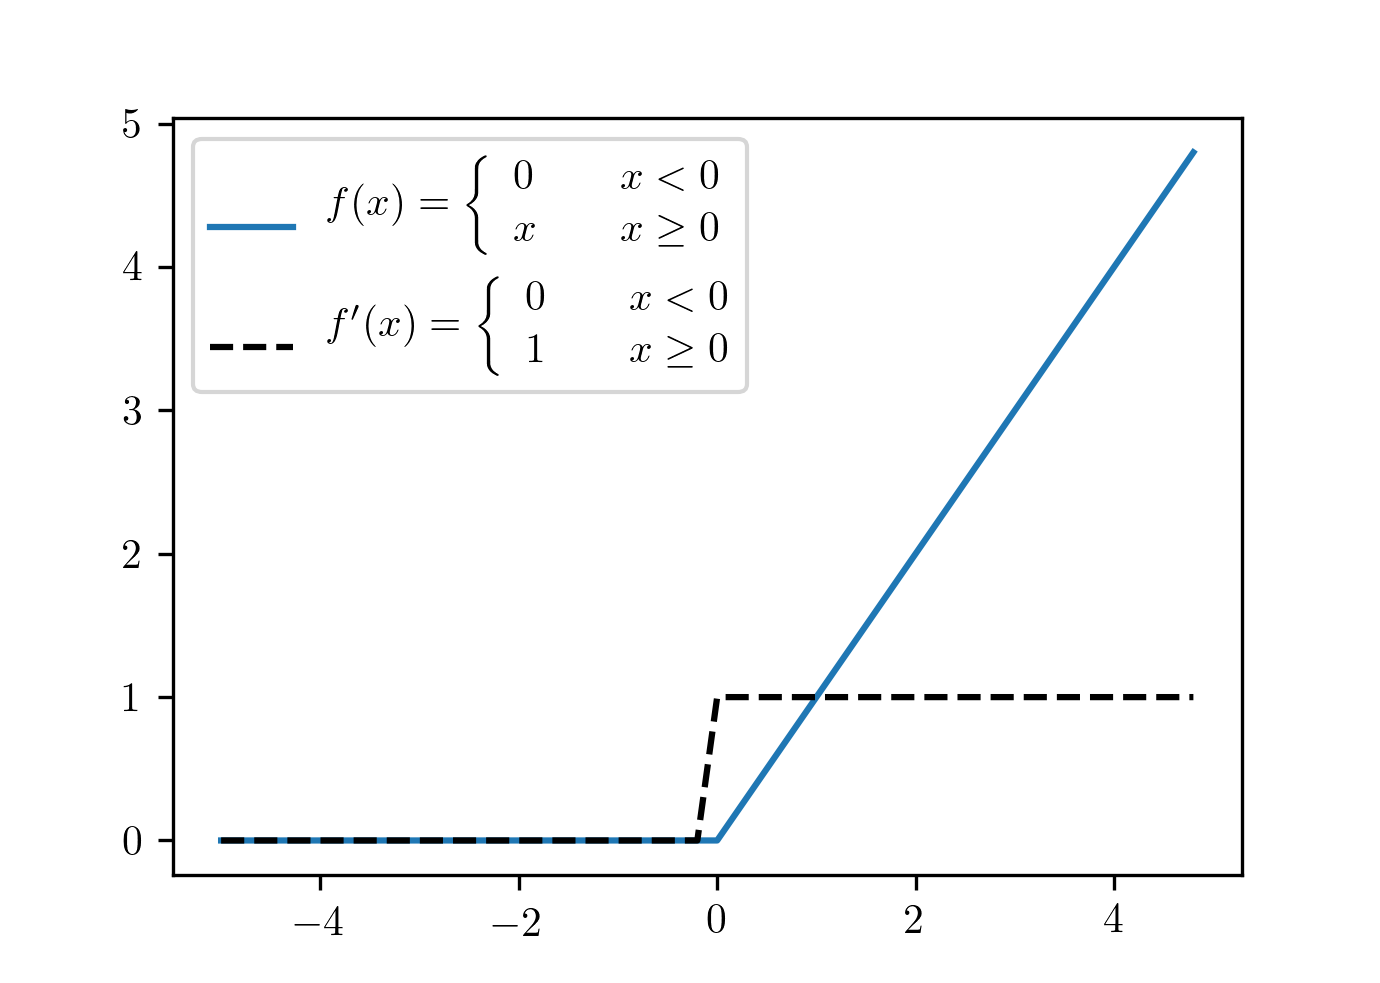
\includegraphics[scale=1]{myFiles/myImages/ReLU.png}
                    \caption{ReLU Graph}
                    \label{fig:ReLU Function}
                \end{figure}

            \subsubsection{ELU}
            ELU is very similar to ReLU, hence can be a good alternative to ReLU. The difference between both is that ELU can be scaled and produces negative output for negative values of the input. However, the negative output does saturate given a large enough negative input. The function and its derivative can be represented by the following mathematical equation and Figure \ref{fig:ELU Function}, where $\alpha = 1$.
            
                \newpage\begin{figure}
                    \centering
                    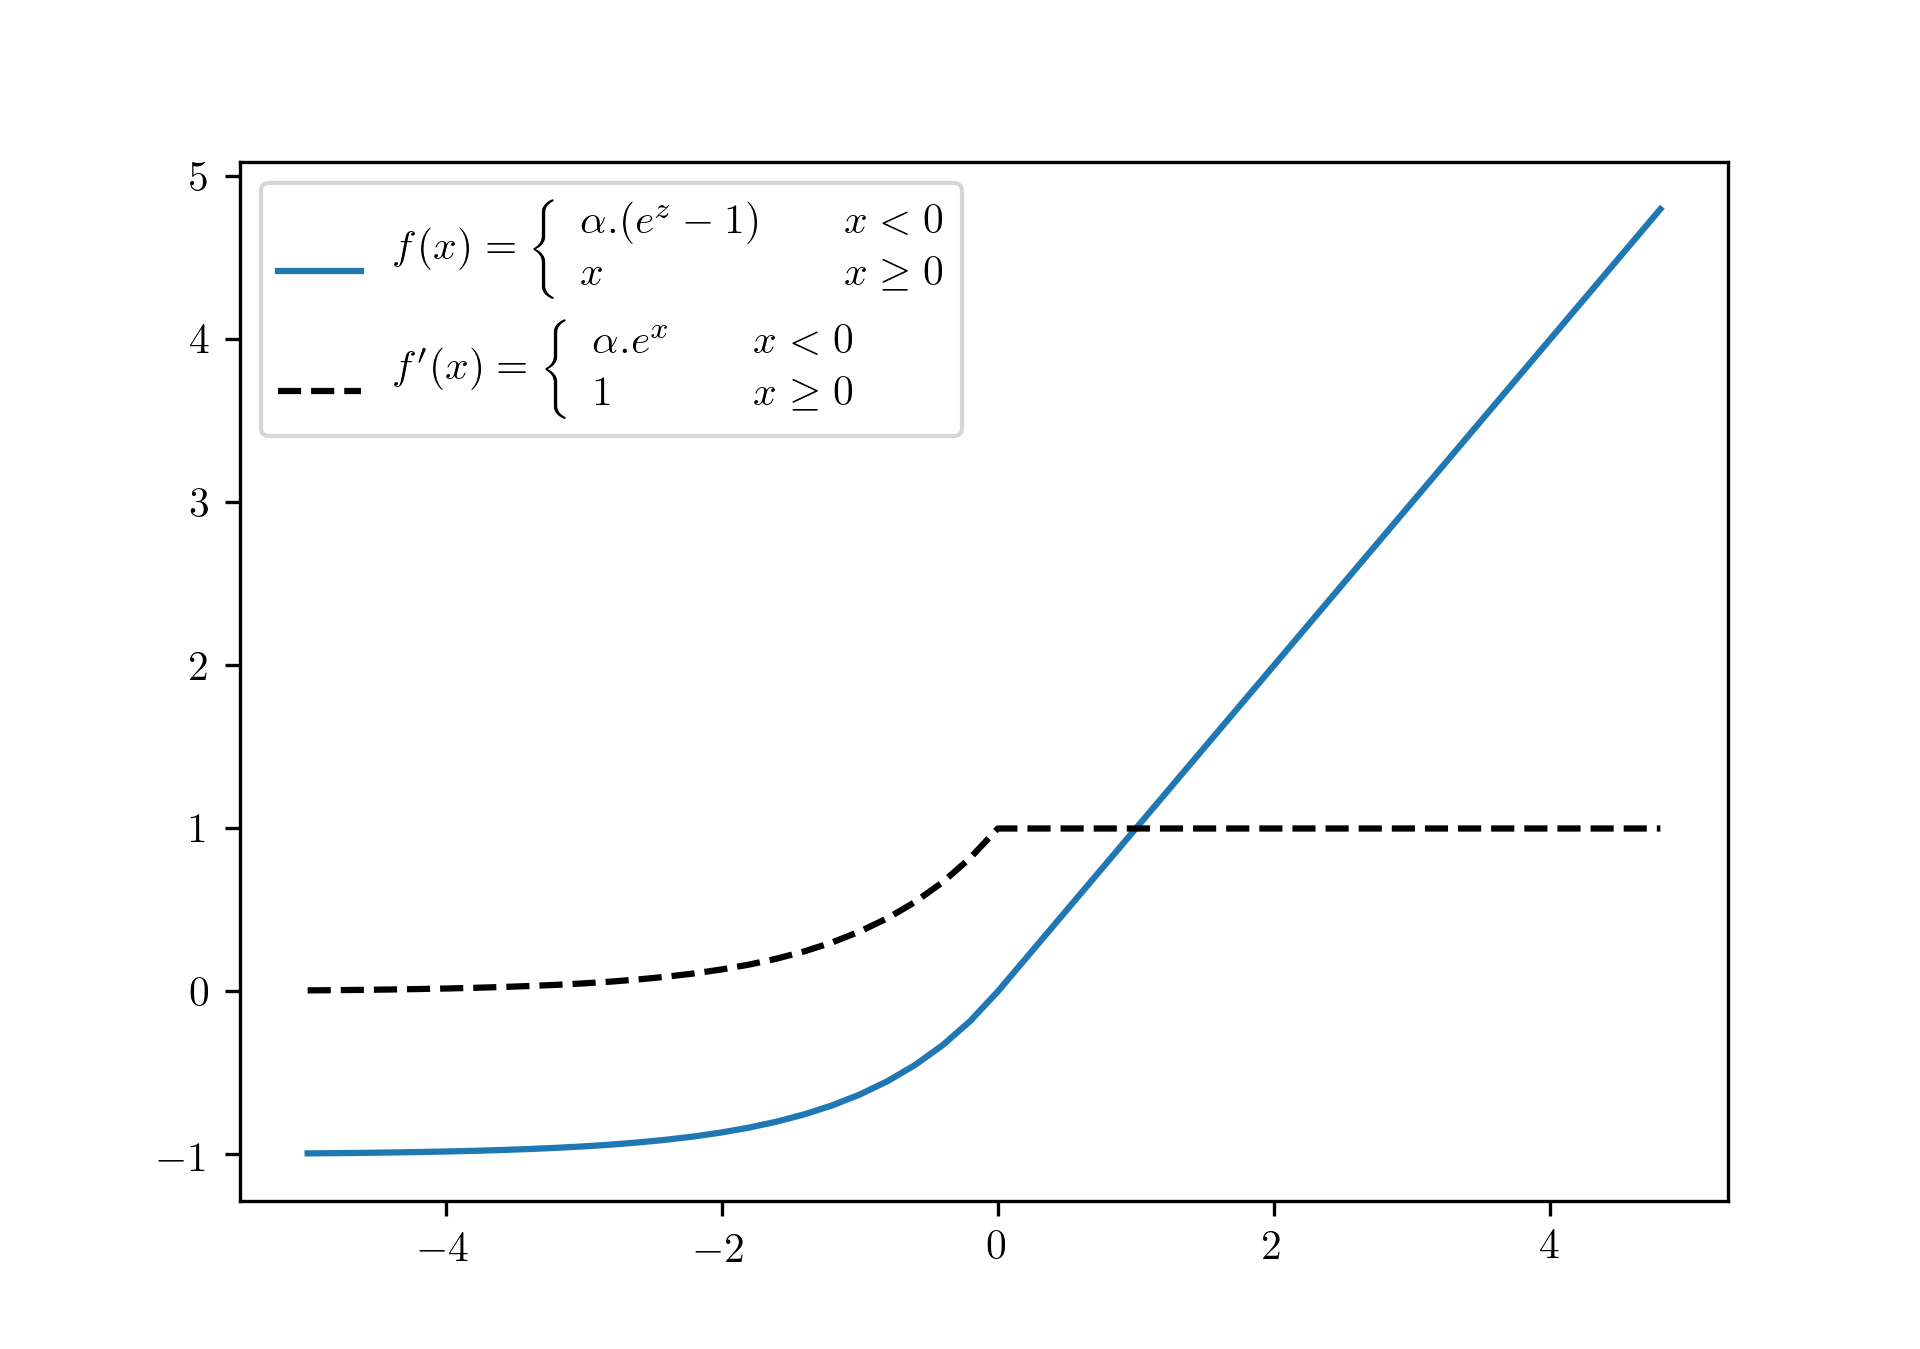
\includegraphics[scale=0.75]{myFiles/myImages/ELU.png}
                    \caption{ELU Graph}
                    \label{fig:ELU Function}
                \end{figure}

            \subsubsection{Hyperbolic Tangent}
            The output of the hyperbolic tangent function is similar to the sigmoid function, such that the output is mapped between 2 values, $-1$ and $1$. As compared to the sigmoid function, the hyperbolic tangent function has a steeper gradient. The function and its derivative can be represented by the following mathematical equation and Figure \ref{fig:tanh Function}.
            
                \begin{figure}[h]
                    \centering
                    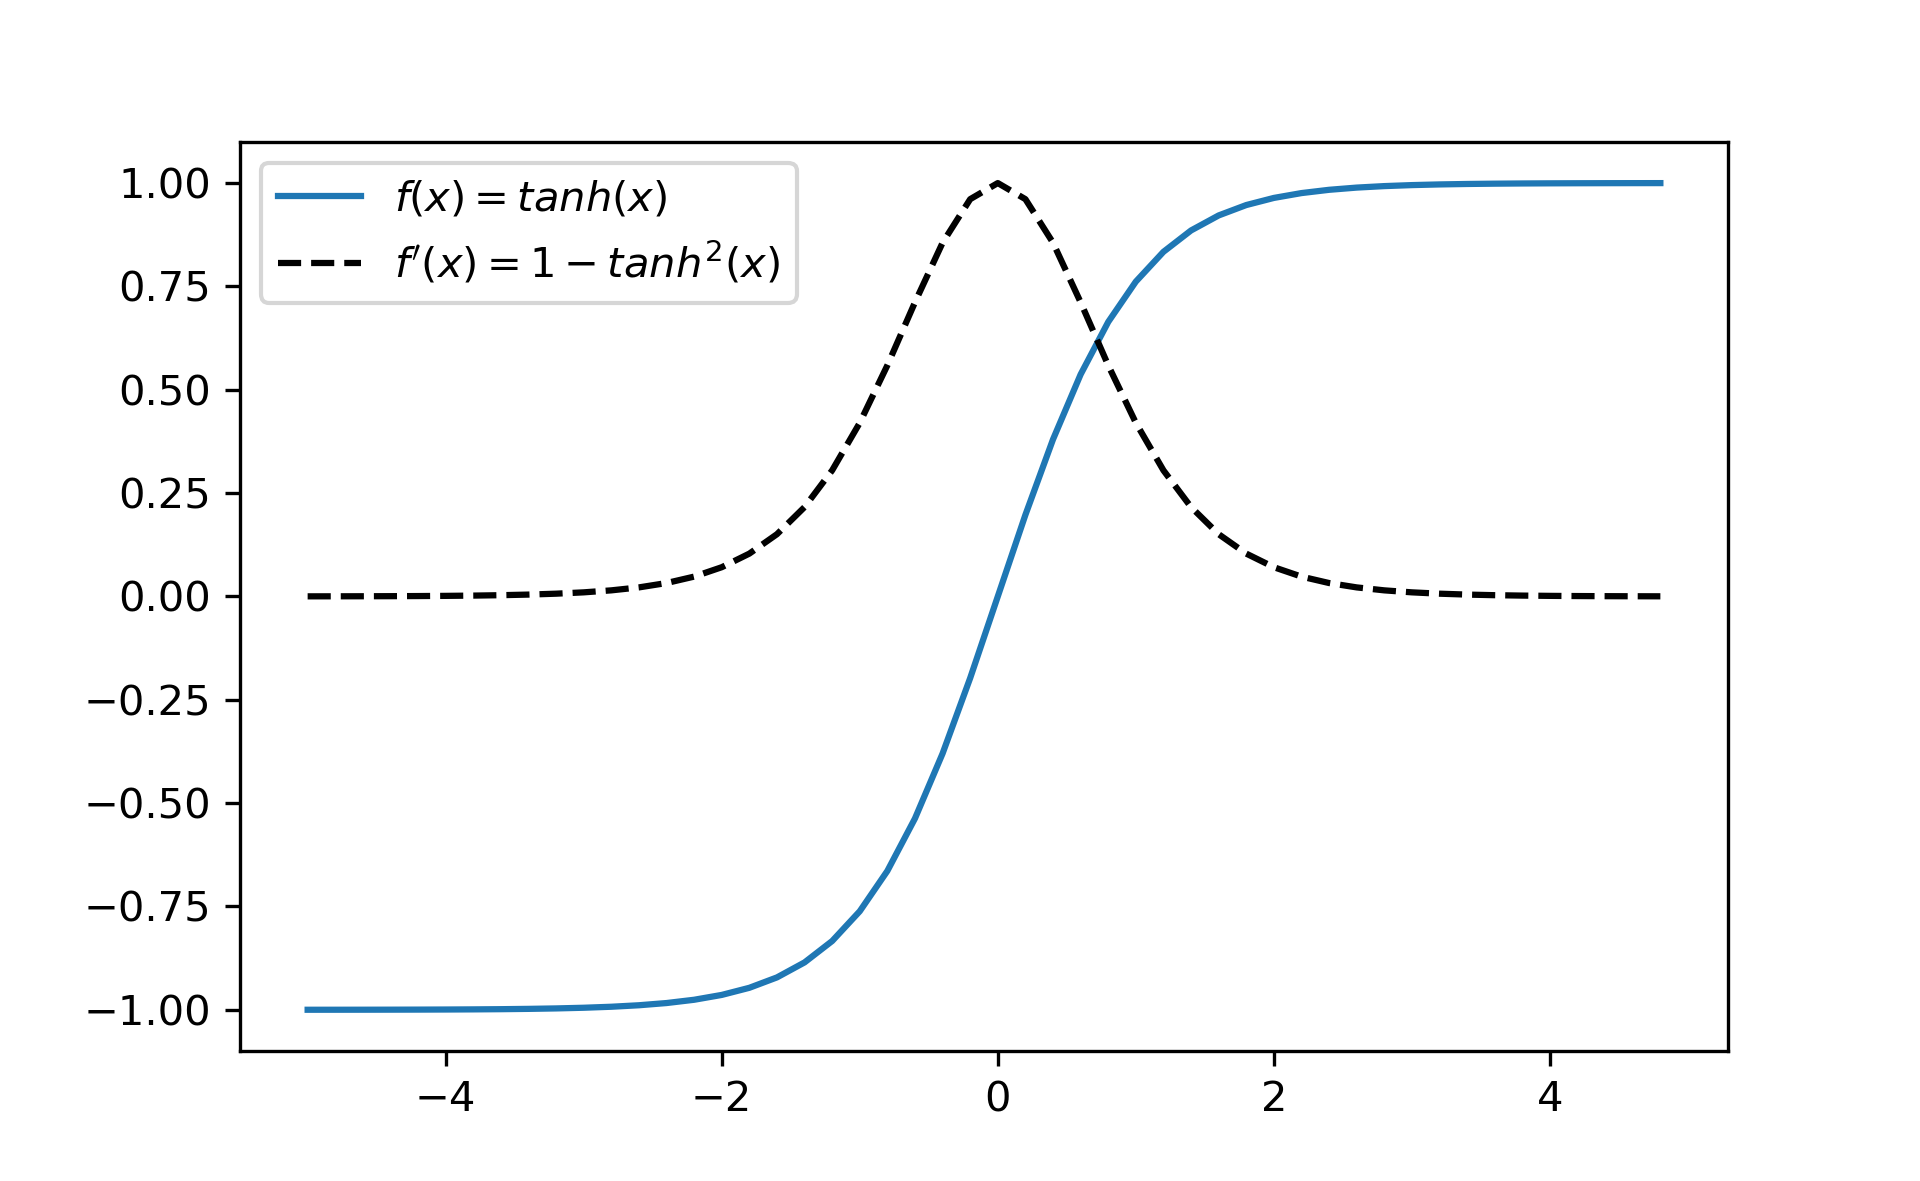
\includegraphics[scale=0.75]{myFiles/myImages/tanh.png}
                    \caption{tanh(x) Graph}
                    \label{fig:tanh Function}
                \end{figure}


        \newpage\subsection{Loss Function}
        The lost function is a measurement hyperparameter, to determine the amount of error between the predicted output and the actual output of the neural network. Choosing the correct loss function, can affect how well the model is viewed. 

            \bigskip\noindent 
            Some common examples of the loss function are:
            \begin{itemize}
                \item Binary Cross Entropy
                \item Mean Square Error
                \item Sparse Categorical Cross Entropy
            \end{itemize}
            The selection of which function to use as a measurement is dependent the what the problem is. 

        \subsection{Optimizer}
        Since the loss function is used to determine the capability of the neural network, the question of can the loss be reduced arises. This is where the optimizer helps. The optimizer role is to find the global minimum of the loss function. This is done by using the chain rule to back propagate, modifying the weights of the neural network. 
        
            \bigskip\noindent 
            Some common examples of the optimizer are:
            \begin{itemize}
                \item Adam
                \item RMSProp
                \item Stochastic Gradient Descent
            \end{itemize}

        \subsection{Epoch}
        Epochs represent the amount of times the neural networks see the training data. Depending on the complexity of the data set, a high number of epochs might result in overfitting. This means the trained model will do particularly well in evaluating the trained data set, but once it is evaluated using the testing data, the model performs poorly. This can be better illustrated in a Figure \ref{fig:Fitting} for under-fitting, optimal-fitting and over-fitting.
        
            \begin{figure}[h]
                \centering
                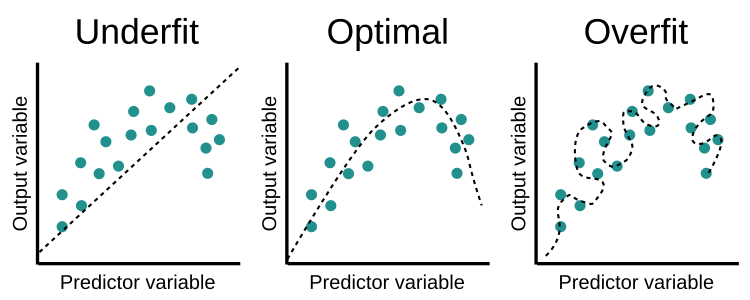
\includegraphics[scale=1]{myFiles/myImages/fitting.png}
                \caption{Fitting}
                \label{fig:Fitting}
            \end{figure}

        \newpage\subsection{Batch Size}
        Batch size is the number of samples that are passed to the network at once. Generally, the larger the batch size, the faster the neural network completes each epoch during training. However, if the batch size is too large, the quality of the neural network may degrade, as it is unable to generalize on the data it has not seen before.
        
        \subsection{Number of Hidden Layers}
        The number of hidden layers refer to the number of layers between the input and output layers.
        
        \subsection{Number of Neurons}
        The number of neurons per layer can differ and should be optimized depending on the usage of the neural network.

        \subsection{Dropout}
        Dropout is a regularization technique to prevent over fitting. Dropout removes some neurons in the layers to prevent the over-reliant on any neuron.

    \newpage\section{Overview of Neural Network}
    With the knowledge of the neural network and its hyperparameters, the flow of how to train and validate a neural network can be discussed. After the pre-processing of the data, the data has to be split into 2 groups, the training set and validation set. 
    
        \bigskip\noindent
        The training and validation data can be defined as follows:
        \begin{itemize}
             \item Training data: Data from a data set which the neural network sees and uses for pattern recognition. 
            \item Validation data: Data from a data set which is not seen by the network, which is used to test the accuracy of train model to provide further insides of the neural network, so that some hyperparameter tuning can be done
        \end{itemize}
        
        \bigskip\noindent
        To train a neural network based on the data set, the recommended practice is to train the model with 80\% of the data set and test with 20\% shown as pre-processing in Figure \ref{fig: Neural Network Flowchart}. This will allow for cross-validation if needed. Once the data is split into groups, it can then be used to train the neural network as shown. A model will be deployed as a trained model and can be validated with the validation set. If the results are not satisfactory, the hyperparameters have to be tuned and the model will have to be retained. In Figure \ref{fig: Neural Network Flowchart}, shows  the overview of how the neural network is trained and validated.
        
        \bigskip\begin{figure}[h]
            \centering
            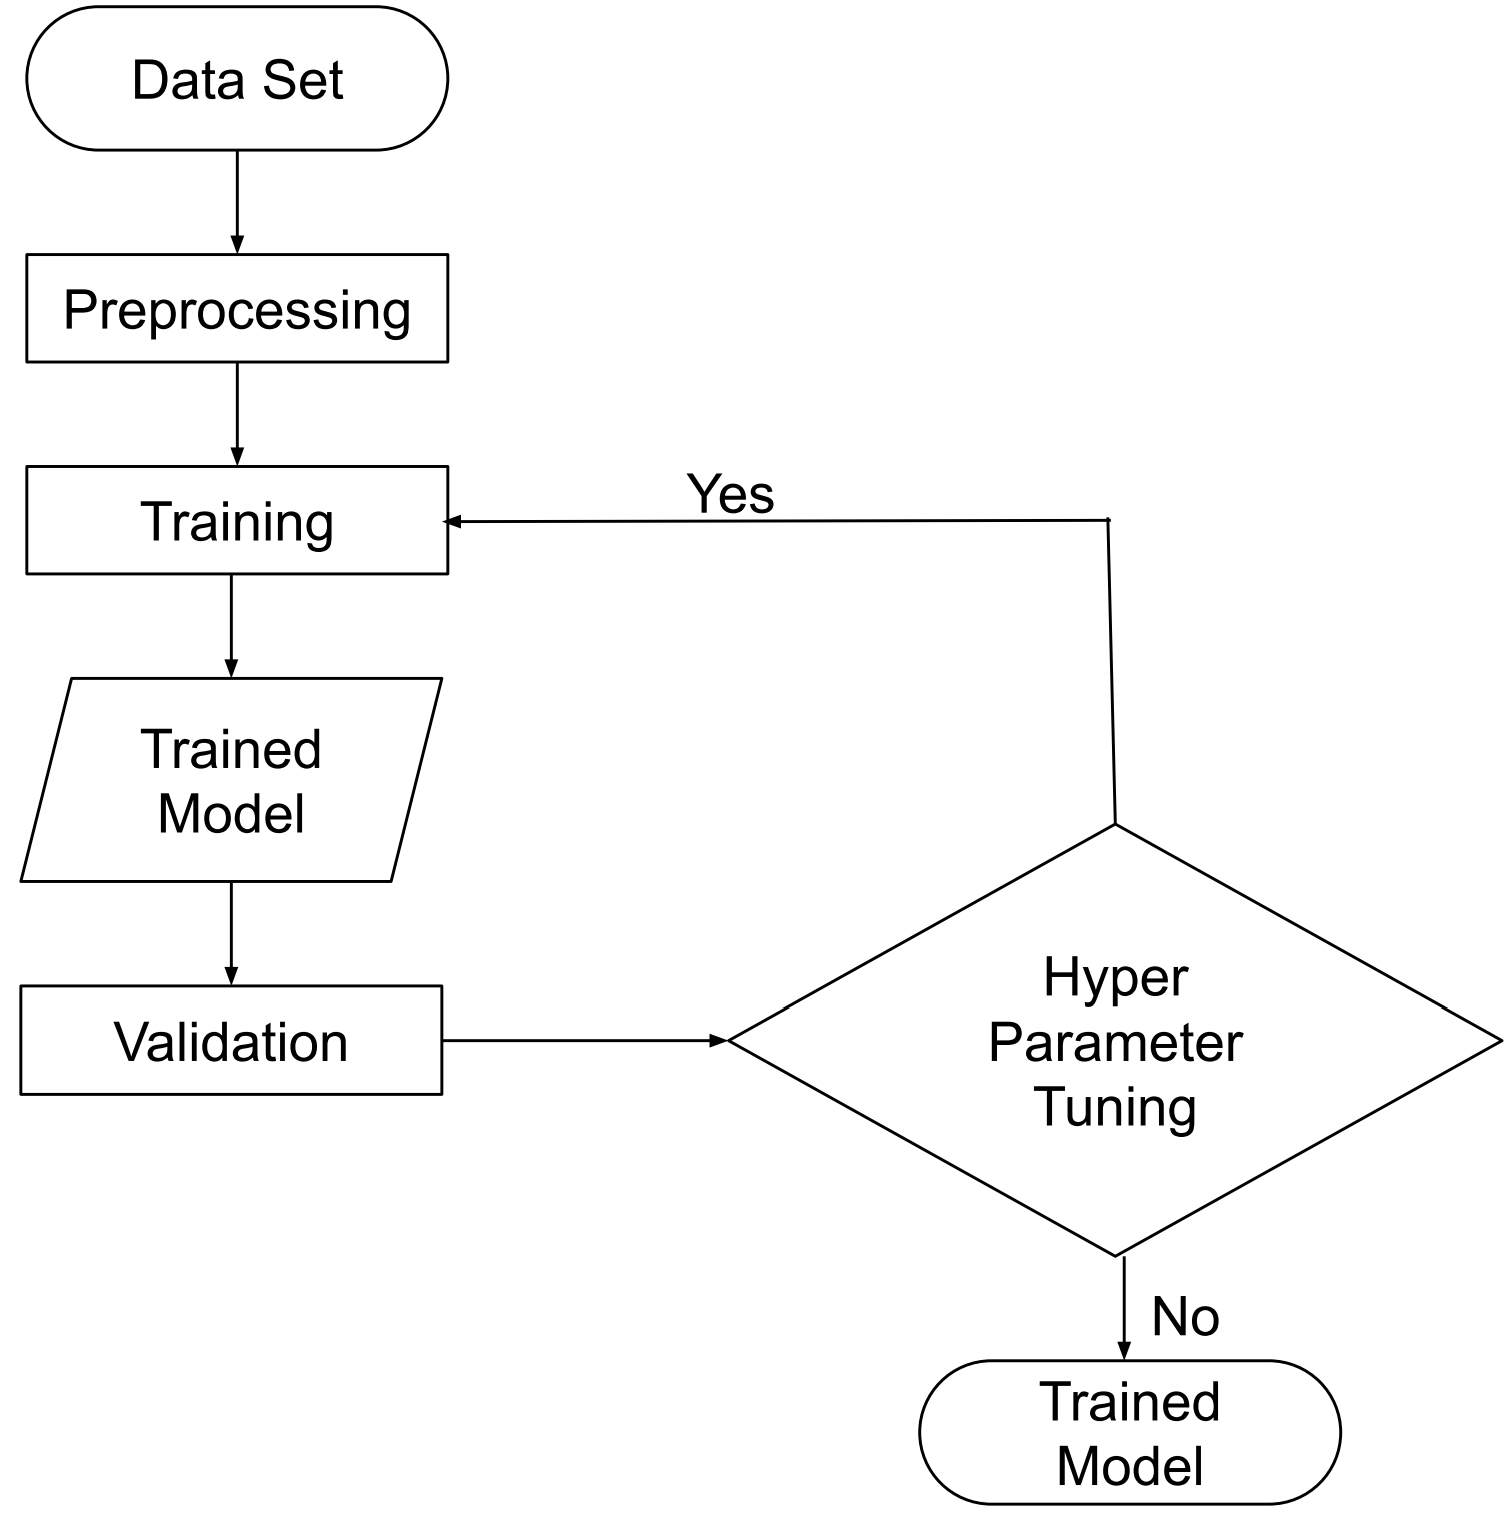
\includegraphics[scale=0.4]{myFiles/myImages/Neural_Network_Flowchart.png}
            \caption{Neural Network Flowchart}
            \label{fig: Neural Network Flowchart}
        \end{figure}
        
        \noindent
        However, due to the limited set of data and the structure of the files, the method of splitting data into 80\% for training and 20\% for testing, was not adopted. The method of training and testing adopted will be further discussed in Chapter \ref{chapter:results}


\chapter{Results}\label{chapter:results}
In Chapter \ref{chapter:pre-processing}, the pre-processing methodology was discussed. In this chapter, the process and results will be discussed.

    \section{Data Manipulation}\label{section:data manipulation}
    As mentioned in Chapter \ref{chapter:pre-processing}, Section \ref{section:feature of design}, the given data consist of the listed feature and each feature holds a certain value for each register in the data file. There is a total of 13 data files given and 12 were used to train, while 1 was used to test. Prior to training, the python module "pandas”\cite{mckinney-proc-scipy-2010} was used to implement the additional feature methods in Section \ref{subsection:methodology of additional features}. The data in 12 training files is then collated into a single collective file. The feature "xx state ff" was subsequently removed from the collated training file and the test file and stored as the target for the neural network. The feature "xx good SN" was dropped as mentioned in Chapter \ref{chapter:pre-processing}, as it is not a feature the neural network should rely on. The data were then scaled using the scaling process.

        \subsection{Implementing Additional Features}\label{subsection:implementing additional features}
        To test which of the additional features implementation performs the best, a neural network was set up using a python module "Keras"\cite{chollet2015keras} with the hyperparameters shown in \ref{tab:Neural Network Hyperparameters}.  

            \begin{table}[ht]
                \centering
                \begin{tabular}{|c|c|}
                \hline
                Hyperparameter & Input\\
                \hline
                \hline
                Optimizer & RMSprop  \\
                \hline
                Loss Function & Binary Crossentropy  \\
                \hline
                Batch Size & 12 \\
                \hline
                Epochs & 22\\
                \hline
                Dropout & 0 \\
                \hline
                First Neurons & 66  \\
                \hline
                Hidden Layers & 12  \\
                \hline
                Hidden Neurons & 50  \\
                \hline
                Hidden Layer Activation Function & ReLU\\
                \hline
                Last Activation Function & Sigmoid\\
                \hline
                \end{tabular}
                \caption{Neural Network Hyperparameters}
                \label{tab:Neural Network Hyperparameters}
            \end{table}
            
        \noindent
        The performance of the implementations can be determined by the accuracy scores of the neural network, given by the mathematical expression:
        
        \begin{equation}
            \label{eqn:model accuracy equation}
            \text{Model Accuracy}= \frac{\text{Number of Correctly Predicted Registers}}{\text{Total Number of Registers}}
        \end{equation}
        
        \noindent
        Since this thesis is about identifying state registers, it is interesting to observe the percentage of state accuracy out of all state registers the neural network correctly predicted as well. The mathematical expression is given to be:
        
        \begin{equation}
            \label{eqn:state register accuracy equation}
            \text{State Register Accuracy}= \frac{\text{Number of Correctly Predicted State Registers}}{\text{Total Number of State Registers}}          
        \end{equation}

        \noindent
        The hyperparameters shown in Table \ref{tab:Neural Network Hyperparameters} were chosen based on the previous experimental runs of using the hyperparameter tuning module "Talos"\cite{Talos}. Previous experimental runs' hyerparamters tested are shown in Table \ref{tab:Talos Parameters}, refer to Section \ref{Talos Tunning} for detailed explanation of "Talos". 
        
                \begin{table}[ht]
                \centering
                \begin{tabular}{|c|c|}
                \hline
                Hyperparameter & Input\\
                \hline
                \hline
                Optimizer & Adam, RMSprop  \\
                \hline
                Loss Function & Binary Crossentropy, Sparse Categorical Crossentropy  \\
                \hline
                Batch Size & 12, 24,32\\
                \hline
                Epochs & 10 to 26, increment of 4 per step\\
                \hline
                Dropout & 0, 0.25, 0.5 \\
                \hline
                First Neurons & 10 to 66, increment of 4 per step  \\
                \hline
                Hidden Layers & 1 to 16, increment of 4 per step  \\
                \hline
                Hidden Neurons & 10, 20, 30, 40, 50  \\
                \hline
                Hidden Layer Activation Function & ELU, ReLU\\
                \hline
                Last Activation Function & Sigmoid\\
                \hline
                \end{tabular}
                \caption{Talos Parameters}
                \label{tab:Talos Parameters}
            \end{table}
        \noindent
        
        \bigskip\noindent
        To test which implementation provides the best results, a consistent set of features across all implementations has to be ensured. Hence, the testing of the different implementations was done prior to feature permutation method and sequential feature selection method, but after constant filtering method.
        
        \bigskip\noindent
        12 files for training and 1 file for testing were rotated, with each file training and testing the model 100 times, e.g, files B--N were used to train the neural network while file A was used to test the neural network, followed by files A, C--N were used to train the neural network while file B was used to test the neural network. 
        
        \bigskip\noindent
        The results were stored and the model in "Keras" backend was cleared after every training and testing to ensure previous training and test results does not affect the current run. The average accuracy scores of 100 runs per file were collated and the process was repeated 5 times to ensure consistency. The results of all implementations with the average accuracy after $5 \times 100$ runs is shown in Tables \ref{tab:Model Accuracy No Feature Selection}  and \ref{tab:State Register Accuracy No Feature Selection}.
        

        \bigskip\noindent
        From Table \ref{tab:Model Accuracy No Feature Selection}, it can be observed that the average model accuracy increased substantially up to $12\%$ with either of the other 3 additional features methods of implementation when compared to the original implementation. Taking a benchmark of $70\%$ as "great performance", the implementation "with fastRELIC" and "with Euclidean and fastRELIC", shows only one file performing below that benchmark, while the implementation of "with Euclidean" has 3 files. Comparing the results, it shows a substantial improvement over the original implementation.
        
        \bigskip\noindent
        Using the benchmark of $70\%$ for the state registers accuracy as a "good performance" reference, from Table \ref{tab:State Register Accuracy No Feature Selection} the implementation "with fastRELIC", though has scored a lower average accuracy across all files by $1\%$ compared to "with Euclidean and fastRELIC", it has a total of nine files, one more file that scored above the $70\%$ benchmark. Overall, all three implementations show a substantial improvement in the number of correctly predicted state registers when compared to the original implementation.
 
        \begin{table}
            \centering
            \begin{tabular}{|c|c|c|c|c|}
    \hline
     & \multicolumn{4}{c|}{Model Accuracy}\\
    \cline {2-5}
    File Name & Original & With fastRELIC & With Euclidean & With Euclidean and fastRELIC\\
    \hline
    \hline
    b01\_reset.csv & 0.95 & 0.97 & 0.98 & 0.97\\
    \hline
    b02\_reset.csv & 0.95 & 0.96 & 0.93 & 0.92\\
    \hline
    b04\_reset.csv & 0.56 & 0.80 & 0.98 & 0.99\\
    \hline
    b06\_reset.csv & 1.00 & 1.00 & 1.00 & 1.00\\
    \hline
    b08\_reset.csv & 0.59 & 0.90 & 0.84 & 0.91\\
    \hline
    b09\_reset.csv & 0.57 & 0.72 & 0.62 & 0.73\\
    \hline
    b10\_reset.csv & 0.73 & 0.79 & 0.76 & 0.83\\
    \hline
    b14\_reset.csv & 0.57 & 0.67 & 0.61 & 0.67\\
    \hline
    completogpio.csv & 0.84 & 0.89 & 0.86 & 0.87\\
    \hline
    FSM.csv & 0.64 & 0.80 & 0.72 & 0.84\\
    \hline
    MEMORY\_INTERFACE.csv & 0.93 & 0.96 & 0.96 & 0.96\\
    \hline
    spi\_axi\_master.csv & 0.98 & 0.97 & 0.96 & 0.92\\
    \hline
    uart.csv & 0.45 & 0.72 & 0.56 & 0.70\\
    \hline
    \hline
    average & 0.75 & 0.86 & 0.83 & 0.87\\
    \hline
\end{tabular}
\caption{Model Accuracy}
\label{tab:Model Accuracy No Feature Selection}


            \bigskip\begin{tabular}{|c|c|c|c|c|}
    \hline
     & \multicolumn{4}{c|}{State Register Accuracy }\\
    \cline {2-5}
    File Name & Original & With fastRELIC & With Euclidean & With Euclidean and fastRELIC\\
    \hline
    \hline
    b01\_reset.csv & 0.92 & 0.95 & 0.96 & 0.95\\
    \hline
    b02\_reset.csv & 0.94 & 0.95 & 0.90 & 0.90\\
    \hline
    b04\_reset.csv & 0.38 & 0.91 & 0.56 & 0.82\\
    \hline
    b06\_reset.csv & 0.99 & 1.00 & 0.99 & 1.00\\
    \hline
    b08\_reset.csv & 0.50 & 0.60 & 0.33 & 0.62\\
    \hline
    b09\_reset.csv & 0.84 & 0.92 & 0.98 & 0.97\\
    \hline
    b10\_reset.csv & 0.88 & 0.86 & 0.93 & 0.87\\
    \hline
    b14\_reset.csv & 0.47 & 0.21 & 0.25 & 0.18\\
    \hline
    completogpio.csv & 0.49 & 0.99 & 1.00 & 1.00\\
    \hline
    FSM.csv & 0.38 & 0.76 & 0.55 & 0.84\\
    \hline
    MEMORY\_INTERFACE.csv & 0.29 & 0.58 & 0.53 & 0.61\\
    \hline
    spi\_axi\_master.csv & 0.33 & 0.52 & 0.73 & 0.67\\
    \hline
    uart.csv & 0.25 & 0.74 & 0.46 & 0.68\\
    \hline
    \hline
    average & 0.59 & 0.77 & 0.71 & 0.78\\
    \hline
\end{tabular}
\caption{State Register Accuracy}
\label{tab:State Register Accuracy No Feature Selection}
        \end{table}
        

    \newpage\section{Feature Selection}\label{section:feature selection result}
        To attempt to improve the results obtained in Table \ref{tab:Model Accuracy No Feature Selection} and \ref{tab:State Register Accuracy No Feature Selection} and reduce the training time, different methods of feature filtering were implemented.
    
        \subsection{Constant Filtering}
        Using the constant filtering method, on the data sets, the constant feature "Degree" was removed from both training and test data frame.
        
        \subsection{Quasi-Constant Filtering}
        Using the quasi-constant filtering method, with a variance threshold of only $1\%$ more than half of the feature sets were removed. This gave the neural network for feature permutation a very limited set of features to work with, resulting in a very poor performance in initial runs. Hence, the use of this filtering method was not implemented.
        
        \subsection{Feature Permutation}\label{section:feature permutation results}
        To implement feature permutation ensuring consistency, all 13 files were rotated with 12 files training and 1 file testing, repeating for a total of 5 times per file. All training files have their features individually permuted for a 100 times, followed by training the neural network and tested for accuracy with the testing set per permutation. The average accuracy of these 100 permutations per feature is then compared with the original data set, which underwent training and testing the same model for a 100 times for 5 times. The algorithm will then determine if the feature is a hindrance or not based on the explained methodology in section \ref{subsubsection:feature permutation}. Refer to Figure \ref{fig:Feature Permutation Flow Chart} for the flowchart.  
        
        \bigskip\noindent
        From the four implemented methods for additional features (including original), two methods of calculating the importance of a feature was used. 
        
        \subsubsection{Determining Feature Importance Method 1}\label{subsection:determining feature importance 1}
        The first method can be expressed in ratio, using the following equations:
        
        \begin{equation}
            \label{eqn:ratio model accuracy}
            R_n(A_{original}, A_{permuted})= \frac{A_{original}}{A_{permuted}}
        \end{equation}
        \begin{equation}
            \label{ration state register accuracy}
            SRR_n(SRA_{original}, SRA_{permuted})= \frac{SRA_{original}}{SRA_{permuted}}
        \end{equation}
        
        \bigskip\noindent
        Where $n$ is the feature, $R_n$ is the ratio between the Model Accuracy(\ref{eqn:model accuracy equation}) of the original feature and permuted features, $SRR_n$ is the ratio between the State Register Accuracy(\ref{eqn:state register accuracy equation}) of the original features and permuted features.
        
        \bigskip\noindent
        The ratio for both equations, can then be interpreted by:
                \begin{table}[ht]
                    \centering
                    \begin{tabular}{|c|c|c|}
                    \hline
                    $R_n<1$ & $SRR_n<1$ & Feature Hindrance\\
                    \hline
                    $R_n=1$ & $SRR_n=1$ & Feature Hindrance\\
                    \hline
                    $R_n>1$ & $SRR_n>1$ & Feature Important\\
                    \hline
                    \end{tabular}
                    \caption{Ratio Interpretation}
                    \label{tab: Ratio Interpretation}
                \end{table}
    
        \bigskip\noindent
        The ratios was calculated by averaging across all the files and runs per feature per implementation method, which is illustrated in Figure \ref{fig:Model Accuracy Ratio ($R_n$) Per Feature} and Figure \ref{fig:Model Accuracy: State Register Ratio ($SRR_n$) Per Feature}.
        

        \newpage\begin{figure*}
            \centering
            % GNUPLOT: LaTeX picture with Postscript
\begingroup
  \makeatletter
  \providecommand\color[2][]{%
    \GenericError{(gnuplot) \space\space\space\@spaces}{%
      Package color not loaded in conjunction with
      terminal option `colourtext'%
    }{See the gnuplot documentation for explanation.%
    }{Either use 'blacktext' in gnuplot or load the package
      color.sty in LaTeX.}%
    \renewcommand\color[2][]{}%
  }%
  \providecommand\includegraphics[2][]{%
    \GenericError{(gnuplot) \space\space\space\@spaces}{%
      Package graphicx or graphics not loaded%
    }{See the gnuplot documentation for explanation.%
    }{The gnuplot epslatex terminal needs graphicx.sty or graphics.sty.}%
    \renewcommand\includegraphics[2][]{}%
  }%
  \providecommand\rotatebox[2]{#2}%
  \@ifundefined{ifGPcolor}{%
    \newif\ifGPcolor
    \GPcolortrue
  }{}%
  \@ifundefined{ifGPblacktext}{%
    \newif\ifGPblacktext
    \GPblacktexttrue
  }{}%
  % define a \g@addto@macro without @ in the name:
  \let\gplgaddtomacro\g@addto@macro
  % define empty templates for all commands taking text:
  \gdef\gplbacktext{}%
  \gdef\gplfronttext{}%
  \makeatother
  \ifGPblacktext
    % no textcolor at all
    \def\colorrgb#1{}%
    \def\colorgray#1{}%
  \else
    % gray or color?
    \ifGPcolor
      \def\colorrgb#1{\color[rgb]{#1}}%
      \def\colorgray#1{\color[gray]{#1}}%
      \expandafter\def\csname LTw\endcsname{\color{white}}%
      \expandafter\def\csname LTb\endcsname{\color{black}}%
      \expandafter\def\csname LTa\endcsname{\color{black}}%
      \expandafter\def\csname LT0\endcsname{\color[rgb]{1,0,0}}%
      \expandafter\def\csname LT1\endcsname{\color[rgb]{0,1,0}}%
      \expandafter\def\csname LT2\endcsname{\color[rgb]{0,0,1}}%
      \expandafter\def\csname LT3\endcsname{\color[rgb]{1,0,1}}%
      \expandafter\def\csname LT4\endcsname{\color[rgb]{0,1,1}}%
      \expandafter\def\csname LT5\endcsname{\color[rgb]{1,1,0}}%
      \expandafter\def\csname LT6\endcsname{\color[rgb]{0,0,0}}%
      \expandafter\def\csname LT7\endcsname{\color[rgb]{1,0.3,0}}%
      \expandafter\def\csname LT8\endcsname{\color[rgb]{0.5,0.5,0.5}}%
    \else
      % gray
      \def\colorrgb#1{\color{black}}%
      \def\colorgray#1{\color[gray]{#1}}%
      \expandafter\def\csname LTw\endcsname{\color{white}}%
      \expandafter\def\csname LTb\endcsname{\color{black}}%
      \expandafter\def\csname LTa\endcsname{\color{black}}%
      \expandafter\def\csname LT0\endcsname{\color{black}}%
      \expandafter\def\csname LT1\endcsname{\color{black}}%
      \expandafter\def\csname LT2\endcsname{\color{black}}%
      \expandafter\def\csname LT3\endcsname{\color{black}}%
      \expandafter\def\csname LT4\endcsname{\color{black}}%
      \expandafter\def\csname LT5\endcsname{\color{black}}%
      \expandafter\def\csname LT6\endcsname{\color{black}}%
      \expandafter\def\csname LT7\endcsname{\color{black}}%
      \expandafter\def\csname LT8\endcsname{\color{black}}%
    \fi
  \fi
    \setlength{\unitlength}{0.0500bp}%
    \ifx\gptboxheight\undefined%
      \newlength{\gptboxheight}%
      \newlength{\gptboxwidth}%
      \newsavebox{\gptboxtext}%
    \fi%
    \setlength{\fboxrule}{0.5pt}%
    \setlength{\fboxsep}{1pt}%
\begin{picture}(9636.00,6802.00)%
    \gplgaddtomacro\gplbacktext{%
      \csname LTb\endcsname%%
      \put(726,1803){\makebox(0,0)[r]{\strut{}$0.9$}}%
      \csname LTb\endcsname%%
      \put(726,2400){\makebox(0,0)[r]{\strut{}$0.95$}}%
      \csname LTb\endcsname%%
      \put(726,2998){\makebox(0,0)[r]{\strut{}$1$}}%
      \csname LTb\endcsname%%
      \put(726,3595){\makebox(0,0)[r]{\strut{}$1.05$}}%
      \csname LTb\endcsname%%
      \put(726,4192){\makebox(0,0)[r]{\strut{}$1.1$}}%
      \csname LTb\endcsname%%
      \put(726,4789){\makebox(0,0)[r]{\strut{}$1.15$}}%
      \csname LTb\endcsname%%
      \put(726,5387){\makebox(0,0)[r]{\strut{}$1.2$}}%
      \csname LTb\endcsname%%
      \put(726,5984){\makebox(0,0)[r]{\strut{}$1.25$}}%
      \csname LTb\endcsname%%
      \put(726,6581){\makebox(0,0)[r]{\strut{}$1.3$}}%
      \csname LTb\endcsname%%
      \put(1975,1671){\rotatebox{30}{\makebox(0,0)[r]{\strut{}average neighbour degree}}}%
      \csname LTb\endcsname%%
      \put(2534,1671){\rotatebox{30}{\makebox(0,0)[r]{\strut{}betweenness centrality}}}%
      \csname LTb\endcsname%%
      \put(3093,1671){\rotatebox{30}{\makebox(0,0)[r]{\strut{}closeness centrality}}}%
      \csname LTb\endcsname%%
      \put(3652,1671){\rotatebox{30}{\makebox(0,0)[r]{\strut{}clustering}}}%
      \csname LTb\endcsname%%
      \put(4210,1671){\rotatebox{30}{\makebox(0,0)[r]{\strut{}degree}}}%
      \csname LTb\endcsname%%
      \put(4769,1671){\rotatebox{30}{\makebox(0,0)[r]{\strut{}degree centrality}}}%
      \csname LTb\endcsname%%
      \put(5328,1671){\rotatebox{30}{\makebox(0,0)[r]{\strut{}has feedback path}}}%
      \csname LTb\endcsname%%
      \put(5887,1671){\rotatebox{30}{\makebox(0,0)[r]{\strut{}katz}}}%
      \csname LTb\endcsname%%
      \put(6445,1671){\rotatebox{30}{\makebox(0,0)[r]{\strut{}load centrality}}}%
      \csname LTb\endcsname%%
      \put(7004,1671){\rotatebox{30}{\makebox(0,0)[r]{\strut{}outdegree}}}%
      \csname LTb\endcsname%%
      \put(7563,1671){\rotatebox{30}{\makebox(0,0)[r]{\strut{}pagerank}}}%
      \csname LTb\endcsname%%
      \put(8122,1671){\rotatebox{30}{\makebox(0,0)[r]{\strut{}Euclidean}}}%
      \csname LTb\endcsname%%
      \put(8680,1671){\rotatebox{30}{\makebox(0,0)[r]{\strut{}fastRELIC}}}%
    }%
    \gplgaddtomacro\gplfronttext{%
      \csname LTb\endcsname%%
      \put(8252,6408){\makebox(0,0)[r]{\strut{}Orignal}}%
      \csname LTb\endcsname%%
      \put(8252,6188){\makebox(0,0)[r]{\strut{}With fastRELIC}}%
      \csname LTb\endcsname%%
      \put(8252,5968){\makebox(0,0)[r]{\strut{}With Euclidean}}%
      \csname LTb\endcsname%%
      \put(8252,5748){\makebox(0,0)[r]{\strut{}With Euclidean and fastRELIC}}%
    }%
    \gplbacktext
    \put(0,0){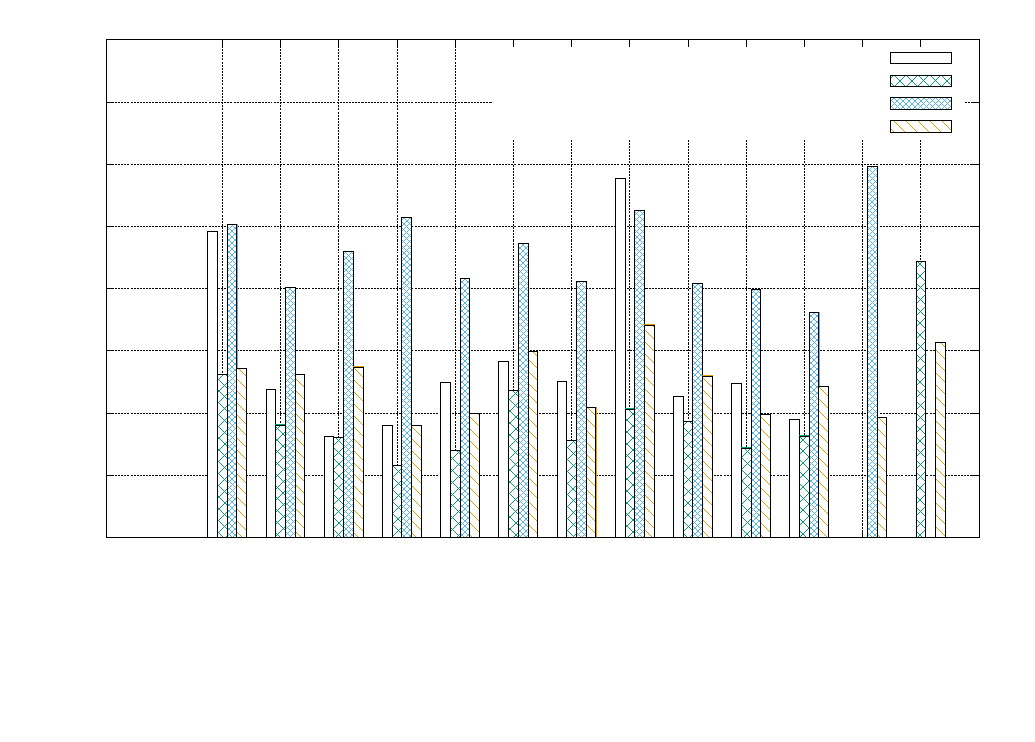
\includegraphics{myFiles/myLatex/Feature_Permutation/FeaturePermutation_ratio.eps}}%
    \gplfronttext
  \end{picture}%
\endgroup

            \caption{Model Accuracy Ratio ($R_n$) Per Feature}
            \label{fig:Model Accuracy Ratio ($R_n$) Per Feature}
        \end{figure*}
        
        \noindent
        In Figure \ref{fig:Model Accuracy Ratio ($R_n$) Per Feature}, focusing on the primary(non-additional) features, it shows general inconsistency across the different implementations, with different implementation viewing different features as important, referencing Table \ref{tab: Ratio Interpretation}. Additionally, with the additional feature(s) implementations, the importance of other features were significantly affected as illustrated. If features below 1 are removed from the respective implementations, this will drastically affect the neural network for the respective implementation in a negative way. Hence, further exploration is needed due to the lack of a clear trend of which features are of lesser importance.
        
        \bigskip\noindent
        Though there is a general inconsistency in feature importance as shown in Figure \ref{fig:Model Accuracy Ratio ($R_n$) Per Feature}, the 3 features which are above the value of 1 across all implementations are "average neighbour degree", "degree centrality” and "katz". Therefore, a conclusion of these 3 features being high importance can be drawn based on $R_n$.
        
        \newpage\begin{figure*}
            \centering
            % GNUPLOT: LaTeX picture with Postscript
\begingroup
  \makeatletter
  \providecommand\color[2][]{%
    \GenericError{(gnuplot) \space\space\space\@spaces}{%
      Package color not loaded in conjunction with
      terminal option `colourtext'%
    }{See the gnuplot documentation for explanation.%
    }{Either use 'blacktext' in gnuplot or load the package
      color.sty in LaTeX.}%
    \renewcommand\color[2][]{}%
  }%
  \providecommand\includegraphics[2][]{%
    \GenericError{(gnuplot) \space\space\space\@spaces}{%
      Package graphicx or graphics not loaded%
    }{See the gnuplot documentation for explanation.%
    }{The gnuplot epslatex terminal needs graphicx.sty or graphics.sty.}%
    \renewcommand\includegraphics[2][]{}%
  }%
  \providecommand\rotatebox[2]{#2}%
  \@ifundefined{ifGPcolor}{%
    \newif\ifGPcolor
    \GPcolortrue
  }{}%
  \@ifundefined{ifGPblacktext}{%
    \newif\ifGPblacktext
    \GPblacktexttrue
  }{}%
  % define a \g@addto@macro without @ in the name:
  \let\gplgaddtomacro\g@addto@macro
  % define empty templates for all commands taking text:
  \gdef\gplbacktext{}%
  \gdef\gplfronttext{}%
  \makeatother
  \ifGPblacktext
    % no textcolor at all
    \def\colorrgb#1{}%
    \def\colorgray#1{}%
  \else
    % gray or color?
    \ifGPcolor
      \def\colorrgb#1{\color[rgb]{#1}}%
      \def\colorgray#1{\color[gray]{#1}}%
      \expandafter\def\csname LTw\endcsname{\color{white}}%
      \expandafter\def\csname LTb\endcsname{\color{black}}%
      \expandafter\def\csname LTa\endcsname{\color{black}}%
      \expandafter\def\csname LT0\endcsname{\color[rgb]{1,0,0}}%
      \expandafter\def\csname LT1\endcsname{\color[rgb]{0,1,0}}%
      \expandafter\def\csname LT2\endcsname{\color[rgb]{0,0,1}}%
      \expandafter\def\csname LT3\endcsname{\color[rgb]{1,0,1}}%
      \expandafter\def\csname LT4\endcsname{\color[rgb]{0,1,1}}%
      \expandafter\def\csname LT5\endcsname{\color[rgb]{1,1,0}}%
      \expandafter\def\csname LT6\endcsname{\color[rgb]{0,0,0}}%
      \expandafter\def\csname LT7\endcsname{\color[rgb]{1,0.3,0}}%
      \expandafter\def\csname LT8\endcsname{\color[rgb]{0.5,0.5,0.5}}%
    \else
      % gray
      \def\colorrgb#1{\color{black}}%
      \def\colorgray#1{\color[gray]{#1}}%
      \expandafter\def\csname LTw\endcsname{\color{white}}%
      \expandafter\def\csname LTb\endcsname{\color{black}}%
      \expandafter\def\csname LTa\endcsname{\color{black}}%
      \expandafter\def\csname LT0\endcsname{\color{black}}%
      \expandafter\def\csname LT1\endcsname{\color{black}}%
      \expandafter\def\csname LT2\endcsname{\color{black}}%
      \expandafter\def\csname LT3\endcsname{\color{black}}%
      \expandafter\def\csname LT4\endcsname{\color{black}}%
      \expandafter\def\csname LT5\endcsname{\color{black}}%
      \expandafter\def\csname LT6\endcsname{\color{black}}%
      \expandafter\def\csname LT7\endcsname{\color{black}}%
      \expandafter\def\csname LT8\endcsname{\color{black}}%
    \fi
  \fi
    \setlength{\unitlength}{0.0500bp}%
    \ifx\gptboxheight\undefined%
      \newlength{\gptboxheight}%
      \newlength{\gptboxwidth}%
      \newsavebox{\gptboxtext}%
    \fi%
    \setlength{\fboxrule}{0.5pt}%
    \setlength{\fboxsep}{1pt}%
\begin{picture}(9636.00,6802.00)%
    \gplgaddtomacro\gplbacktext{%
      \csname LTb\endcsname%%
      \put(594,1803){\makebox(0,0)[r]{\strut{}$0.5$}}%
      \csname LTb\endcsname%%
      \put(594,2998){\makebox(0,0)[r]{\strut{}$1$}}%
      \csname LTb\endcsname%%
      \put(594,4192){\makebox(0,0)[r]{\strut{}$1.5$}}%
      \csname LTb\endcsname%%
      \put(594,5387){\makebox(0,0)[r]{\strut{}$2$}}%
      \csname LTb\endcsname%%
      \put(594,6581){\makebox(0,0)[r]{\strut{}$2.5$}}%
      \csname LTb\endcsname%%
      \put(1861,1671){\rotatebox{30}{\makebox(0,0)[r]{\strut{}average neighbour degree}}}%
      \csname LTb\endcsname%%
      \put(2429,1671){\rotatebox{30}{\makebox(0,0)[r]{\strut{}betweenness centrality}}}%
      \csname LTb\endcsname%%
      \put(2996,1671){\rotatebox{30}{\makebox(0,0)[r]{\strut{}closeness centrality}}}%
      \csname LTb\endcsname%%
      \put(3564,1671){\rotatebox{30}{\makebox(0,0)[r]{\strut{}clustering}}}%
      \csname LTb\endcsname%%
      \put(4131,1671){\rotatebox{30}{\makebox(0,0)[r]{\strut{}degree}}}%
      \csname LTb\endcsname%%
      \put(4699,1671){\rotatebox{30}{\makebox(0,0)[r]{\strut{}degree centrality}}}%
      \csname LTb\endcsname%%
      \put(5266,1671){\rotatebox{30}{\makebox(0,0)[r]{\strut{}has feedback path}}}%
      \csname LTb\endcsname%%
      \put(5834,1671){\rotatebox{30}{\makebox(0,0)[r]{\strut{}katz}}}%
      \csname LTb\endcsname%%
      \put(6401,1671){\rotatebox{30}{\makebox(0,0)[r]{\strut{}load centrality}}}%
      \csname LTb\endcsname%%
      \put(6969,1671){\rotatebox{30}{\makebox(0,0)[r]{\strut{}outdegree}}}%
      \csname LTb\endcsname%%
      \put(7536,1671){\rotatebox{30}{\makebox(0,0)[r]{\strut{}pagerank}}}%
      \csname LTb\endcsname%%
      \put(8104,1671){\rotatebox{30}{\makebox(0,0)[r]{\strut{}euclidean}}}%
      \csname LTb\endcsname%%
      \put(8671,1671){\rotatebox{30}{\makebox(0,0)[r]{\strut{}fastRELIC}}}%
    }%
    \gplgaddtomacro\gplfronttext{%
      \csname LTb\endcsname%%
      \put(8252,6408){\makebox(0,0)[r]{\strut{}Original}}%
      \csname LTb\endcsname%%
      \put(8252,6188){\makebox(0,0)[r]{\strut{}With fastRELIC}}%
      \csname LTb\endcsname%%
      \put(8252,5968){\makebox(0,0)[r]{\strut{}With Euclidean}}%
      \csname LTb\endcsname%%
      \put(8252,5748){\makebox(0,0)[r]{\strut{}With Euclidean and fastRELIC}}%
    }%
    \gplbacktext
    \put(0,0){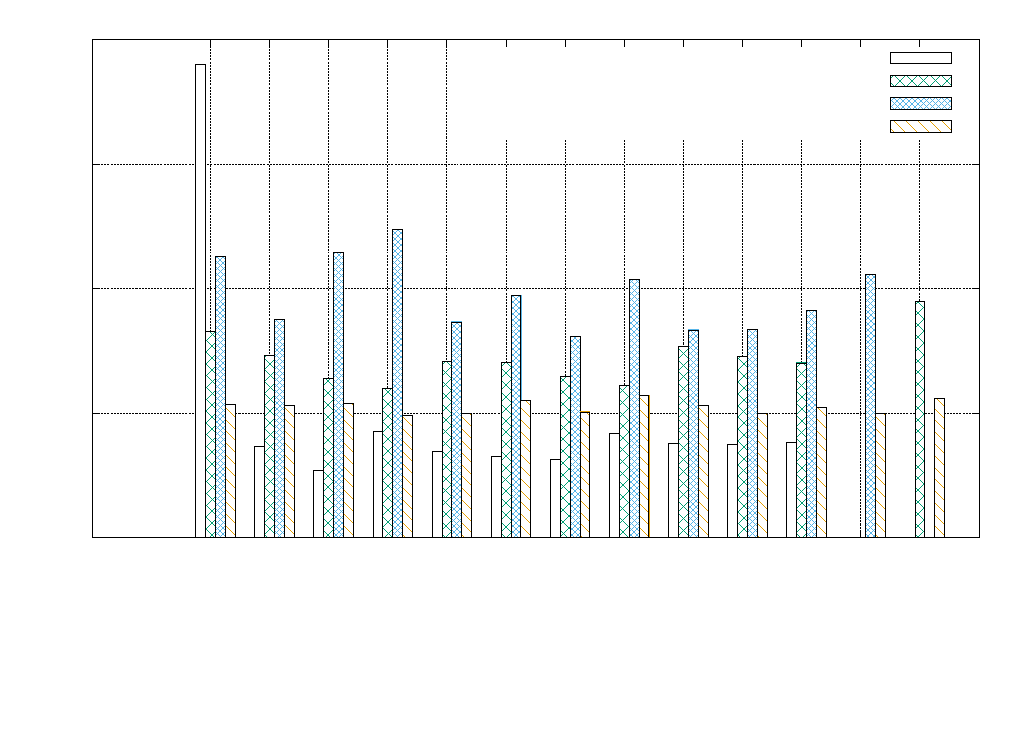
\includegraphics{./Results/Feature_Permutation/statereg_ratio.eps}}%
    \gplfronttext
  \end{picture}%
\endgroup

            \caption{Model Accuracy: State Register Ratio ($SRR_n$) Per Feature}
            \label{fig:Model Accuracy: State Register Ratio ($SRR_n$) Per Feature}
        \end{figure*}
 
        \bigskip\noindent 
        Applying method 1 on the State Register Accuracy instead of the Model Accuracy yields Figure \ref{fig:Model Accuracy: State Register Ratio ($SRR_n$) Per Feature}, which upon first observation seem to be a very different graph, compared to Figure \ref{fig:Model Accuracy Ratio ($R_n$) Per Feature}. This significant value difference can be explained by the amount of state registers in a file. Given that the number of state registers in a file is smaller than the total of all registers type in a file, a value change will cause a significant difference in the final ratio. Therefore, instead of solely focusing on the values, the trend should be taken into consideration as well. Comparing Figure \ref{fig:Model Accuracy: State Register Ratio ($SRR_n$) Per Feature} to Figure \ref{fig:Model Accuracy Ratio ($R_n$) Per Feature}, despite the files "with Euclidean" having significantly higher ratio in Figure \ref{fig:Model Accuracy: State Register Ratio ($SRR_n$) Per Feature} compared to Figure \ref{fig:Model Accuracy Ratio ($R_n$) Per Feature}, the ratio values for each feature remains more than 1, which is similar in both figures. For the file "with fastRELIC", all feature ratio is now above 1 thus, a definite conclusion of those features below the value of 1 in \ref{fig:Model Accuracy Ratio ($R_n$) Per Feature} being less important cannot be drawn.
        
        
        \subsubsection{Determining Feature Importance Method 2}\label{subsection:determining feature importance 2}
        The second method mentioned determines the percentage of feature occurrence across the files to assess feature importance. A counting algorithm is used to count the total amount of times the feature appears after feature permutation selection based on a set of conditions explained in Section \ref{subsubsection:feature permutation}, shown in Table \ref{tab: conditions for filtering}. 
        
        \newpage\noindent
        The conditions are as follows:
            \begin{table}[ht]
                \centering
                \begin{tabular}{|c|c|}
                \hline
                $A_{original}<A_{permuted}$ & Feature Hindrance\\
                \hline
                $A_{original}=A_{permuted}$ & Feature Hindrance\\
                \hline
                $A_{original}>A_{permuted}$, \; with a difference of $> 1\%$  & Feature Important\\
                \hline
                \end{tabular}
                \caption{Conditions for filtering}
                \label{tab: conditions for filtering}
            \end{table}
    
        \noindent
        The percentage of occurrence can be expressed by:
                \begin{equation}
                    \label{eqn:percentage of feature occurrence}
                    C(n)=(\frac{1}{k}\sum_{i=0}^{k} {[f_i = n]})
                \end{equation}
        \bigskip\noindent
        where $n$ is the feature, $k$ is the total amount of runs of all files, thus $k=65$ in this experiment.
        
        \begin{figure*}[hb]
        \centering
            % GNUPLOT: LaTeX picture with Postscript
\begingroup
  \makeatletter
  \providecommand\color[2][]{%
    \GenericError{(gnuplot) \space\space\space\@spaces}{%
      Package color not loaded in conjunction with
      terminal option `colourtext'%
    }{See the gnuplot documentation for explanation.%
    }{Either use 'blacktext' in gnuplot or load the package
      color.sty in LaTeX.}%
    \renewcommand\color[2][]{}%
  }%
  \providecommand\includegraphics[2][]{%
    \GenericError{(gnuplot) \space\space\space\@spaces}{%
      Package graphicx or graphics not loaded%
    }{See the gnuplot documentation for explanation.%
    }{The gnuplot epslatex terminal needs graphicx.sty or graphics.sty.}%
    \renewcommand\includegraphics[2][]{}%
  }%
  \providecommand\rotatebox[2]{#2}%
  \@ifundefined{ifGPcolor}{%
    \newif\ifGPcolor
    \GPcolortrue
  }{}%
  \@ifundefined{ifGPblacktext}{%
    \newif\ifGPblacktext
    \GPblacktexttrue
  }{}%
  % define a \g@addto@macro without @ in the name:
  \let\gplgaddtomacro\g@addto@macro
  % define empty templates for all commands taking text:
  \gdef\gplbacktext{}%
  \gdef\gplfronttext{}%
  \makeatother
  \ifGPblacktext
    % no textcolor at all
    \def\colorrgb#1{}%
    \def\colorgray#1{}%
  \else
    % gray or color?
    \ifGPcolor
      \def\colorrgb#1{\color[rgb]{#1}}%
      \def\colorgray#1{\color[gray]{#1}}%
      \expandafter\def\csname LTw\endcsname{\color{white}}%
      \expandafter\def\csname LTb\endcsname{\color{black}}%
      \expandafter\def\csname LTa\endcsname{\color{black}}%
      \expandafter\def\csname LT0\endcsname{\color[rgb]{1,0,0}}%
      \expandafter\def\csname LT1\endcsname{\color[rgb]{0,1,0}}%
      \expandafter\def\csname LT2\endcsname{\color[rgb]{0,0,1}}%
      \expandafter\def\csname LT3\endcsname{\color[rgb]{1,0,1}}%
      \expandafter\def\csname LT4\endcsname{\color[rgb]{0,1,1}}%
      \expandafter\def\csname LT5\endcsname{\color[rgb]{1,1,0}}%
      \expandafter\def\csname LT6\endcsname{\color[rgb]{0,0,0}}%
      \expandafter\def\csname LT7\endcsname{\color[rgb]{1,0.3,0}}%
      \expandafter\def\csname LT8\endcsname{\color[rgb]{0.5,0.5,0.5}}%
    \else
      % gray
      \def\colorrgb#1{\color{black}}%
      \def\colorgray#1{\color[gray]{#1}}%
      \expandafter\def\csname LTw\endcsname{\color{white}}%
      \expandafter\def\csname LTb\endcsname{\color{black}}%
      \expandafter\def\csname LTa\endcsname{\color{black}}%
      \expandafter\def\csname LT0\endcsname{\color{black}}%
      \expandafter\def\csname LT1\endcsname{\color{black}}%
      \expandafter\def\csname LT2\endcsname{\color{black}}%
      \expandafter\def\csname LT3\endcsname{\color{black}}%
      \expandafter\def\csname LT4\endcsname{\color{black}}%
      \expandafter\def\csname LT5\endcsname{\color{black}}%
      \expandafter\def\csname LT6\endcsname{\color{black}}%
      \expandafter\def\csname LT7\endcsname{\color{black}}%
      \expandafter\def\csname LT8\endcsname{\color{black}}%
    \fi
  \fi
    \setlength{\unitlength}{0.0500bp}%
    \ifx\gptboxheight\undefined%
      \newlength{\gptboxheight}%
      \newlength{\gptboxwidth}%
      \newsavebox{\gptboxtext}%
    \fi%
    \setlength{\fboxrule}{0.5pt}%
    \setlength{\fboxsep}{1pt}%
\begin{picture}(9636.00,6802.00)%
    \gplgaddtomacro\gplbacktext{%
      \csname LTb\endcsname%%
      \put(594,1803){\makebox(0,0)[r]{\strut{}$0.2$}}%
      \csname LTb\endcsname%%
      \put(594,2759){\makebox(0,0)[r]{\strut{}$0.4$}}%
      \csname LTb\endcsname%%
      \put(594,3714){\makebox(0,0)[r]{\strut{}$0.6$}}%
      \csname LTb\endcsname%%
      \put(594,4670){\makebox(0,0)[r]{\strut{}$0.8$}}%
      \csname LTb\endcsname%%
      \put(594,5625){\makebox(0,0)[r]{\strut{}$1$}}%
      \csname LTb\endcsname%%
      \put(594,6581){\makebox(0,0)[r]{\strut{}$1.2$}}%
      \csname LTb\endcsname%%
      \put(1861,1671){\rotatebox{30}{\makebox(0,0)[r]{\strut{}average neighbour degree}}}%
      \csname LTb\endcsname%%
      \put(2429,1671){\rotatebox{30}{\makebox(0,0)[r]{\strut{}betweenness centrality}}}%
      \csname LTb\endcsname%%
      \put(2996,1671){\rotatebox{30}{\makebox(0,0)[r]{\strut{}closeness centrality}}}%
      \csname LTb\endcsname%%
      \put(3564,1671){\rotatebox{30}{\makebox(0,0)[r]{\strut{}clustering}}}%
      \csname LTb\endcsname%%
      \put(4131,1671){\rotatebox{30}{\makebox(0,0)[r]{\strut{}degree}}}%
      \csname LTb\endcsname%%
      \put(4699,1671){\rotatebox{30}{\makebox(0,0)[r]{\strut{}degree centrality}}}%
      \csname LTb\endcsname%%
      \put(5266,1671){\rotatebox{30}{\makebox(0,0)[r]{\strut{}has feedback path}}}%
      \csname LTb\endcsname%%
      \put(5834,1671){\rotatebox{30}{\makebox(0,0)[r]{\strut{}katz}}}%
      \csname LTb\endcsname%%
      \put(6401,1671){\rotatebox{30}{\makebox(0,0)[r]{\strut{}load centrality}}}%
      \csname LTb\endcsname%%
      \put(6969,1671){\rotatebox{30}{\makebox(0,0)[r]{\strut{}outdegree}}}%
      \csname LTb\endcsname%%
      \put(7536,1671){\rotatebox{30}{\makebox(0,0)[r]{\strut{}pagerank}}}%
      \csname LTb\endcsname%%
      \put(8104,1671){\rotatebox{30}{\makebox(0,0)[r]{\strut{}euclidean}}}%
      \csname LTb\endcsname%%
      \put(8671,1671){\rotatebox{30}{\makebox(0,0)[r]{\strut{}fastRELIC}}}%
    }%
    \gplgaddtomacro\gplfronttext{%
      \csname LTb\endcsname%%
      \put(8252,6408){\makebox(0,0)[r]{\strut{}Original}}%
      \csname LTb\endcsname%%
      \put(8252,6188){\makebox(0,0)[r]{\strut{}With fastRELIC}}%
      \csname LTb\endcsname%%
      \put(8252,5968){\makebox(0,0)[r]{\strut{}With Euclidean}}%
      \csname LTb\endcsname%%
      \put(8252,5748){\makebox(0,0)[r]{\strut{}With Euclidean and fastRELIC}}%
    }%
    \gplbacktext
    \put(0,0){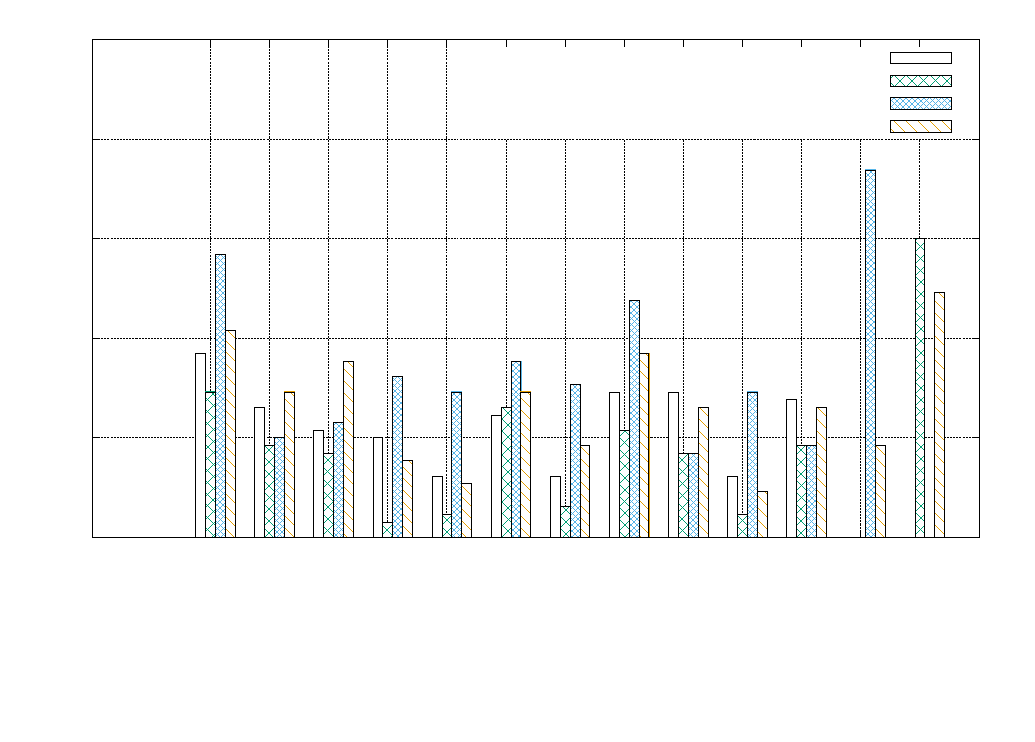
\includegraphics{FeaturePermutation_count}}%
    \gplfronttext
  \end{picture}%
\endgroup

            \caption{Feature Occurrence Percentage: FP Model}
            \label{fig:Feature Occurrence Percentage: FP Model}
        \end{figure*}
        
        \newpage\begin{figure*}[ht]
            % GNUPLOT: LaTeX picture with Postscript
\begingroup
  \makeatletter
  \providecommand\color[2][]{%
    \GenericError{(gnuplot) \space\space\space\@spaces}{%
      Package color not loaded in conjunction with
      terminal option `colourtext'%
    }{See the gnuplot documentation for explanation.%
    }{Either use 'blacktext' in gnuplot or load the package
      color.sty in LaTeX.}%
    \renewcommand\color[2][]{}%
  }%
  \providecommand\includegraphics[2][]{%
    \GenericError{(gnuplot) \space\space\space\@spaces}{%
      Package graphicx or graphics not loaded%
    }{See the gnuplot documentation for explanation.%
    }{The gnuplot epslatex terminal needs graphicx.sty or graphics.sty.}%
    \renewcommand\includegraphics[2][]{}%
  }%
  \providecommand\rotatebox[2]{#2}%
  \@ifundefined{ifGPcolor}{%
    \newif\ifGPcolor
    \GPcolortrue
  }{}%
  \@ifundefined{ifGPblacktext}{%
    \newif\ifGPblacktext
    \GPblacktexttrue
  }{}%
  % define a \g@addto@macro without @ in the name:
  \let\gplgaddtomacro\g@addto@macro
  % define empty templates for all commands taking text:
  \gdef\gplbacktext{}%
  \gdef\gplfronttext{}%
  \makeatother
  \ifGPblacktext
    % no textcolor at all
    \def\colorrgb#1{}%
    \def\colorgray#1{}%
  \else
    % gray or color?
    \ifGPcolor
      \def\colorrgb#1{\color[rgb]{#1}}%
      \def\colorgray#1{\color[gray]{#1}}%
      \expandafter\def\csname LTw\endcsname{\color{white}}%
      \expandafter\def\csname LTb\endcsname{\color{black}}%
      \expandafter\def\csname LTa\endcsname{\color{black}}%
      \expandafter\def\csname LT0\endcsname{\color[rgb]{1,0,0}}%
      \expandafter\def\csname LT1\endcsname{\color[rgb]{0,1,0}}%
      \expandafter\def\csname LT2\endcsname{\color[rgb]{0,0,1}}%
      \expandafter\def\csname LT3\endcsname{\color[rgb]{1,0,1}}%
      \expandafter\def\csname LT4\endcsname{\color[rgb]{0,1,1}}%
      \expandafter\def\csname LT5\endcsname{\color[rgb]{1,1,0}}%
      \expandafter\def\csname LT6\endcsname{\color[rgb]{0,0,0}}%
      \expandafter\def\csname LT7\endcsname{\color[rgb]{1,0.3,0}}%
      \expandafter\def\csname LT8\endcsname{\color[rgb]{0.5,0.5,0.5}}%
    \else
      % gray
      \def\colorrgb#1{\color{black}}%
      \def\colorgray#1{\color[gray]{#1}}%
      \expandafter\def\csname LTw\endcsname{\color{white}}%
      \expandafter\def\csname LTb\endcsname{\color{black}}%
      \expandafter\def\csname LTa\endcsname{\color{black}}%
      \expandafter\def\csname LT0\endcsname{\color{black}}%
      \expandafter\def\csname LT1\endcsname{\color{black}}%
      \expandafter\def\csname LT2\endcsname{\color{black}}%
      \expandafter\def\csname LT3\endcsname{\color{black}}%
      \expandafter\def\csname LT4\endcsname{\color{black}}%
      \expandafter\def\csname LT5\endcsname{\color{black}}%
      \expandafter\def\csname LT6\endcsname{\color{black}}%
      \expandafter\def\csname LT7\endcsname{\color{black}}%
      \expandafter\def\csname LT8\endcsname{\color{black}}%
    \fi
  \fi
    \setlength{\unitlength}{0.0500bp}%
    \ifx\gptboxheight\undefined%
      \newlength{\gptboxheight}%
      \newlength{\gptboxwidth}%
      \newsavebox{\gptboxtext}%
    \fi%
    \setlength{\fboxrule}{0.5pt}%
    \setlength{\fboxsep}{1pt}%
\begin{picture}(9636.00,6802.00)%
    \gplgaddtomacro\gplbacktext{%
      \csname LTb\endcsname%%
      \put(594,1803){\makebox(0,0)[r]{\strut{}$0$}}%
      \csname LTb\endcsname%%
      \put(594,2759){\makebox(0,0)[r]{\strut{}$0.2$}}%
      \csname LTb\endcsname%%
      \put(594,3714){\makebox(0,0)[r]{\strut{}$0.4$}}%
      \csname LTb\endcsname%%
      \put(594,4670){\makebox(0,0)[r]{\strut{}$0.6$}}%
      \csname LTb\endcsname%%
      \put(594,5625){\makebox(0,0)[r]{\strut{}$0.8$}}%
      \csname LTb\endcsname%%
      \put(594,6581){\makebox(0,0)[r]{\strut{}$1$}}%
      \csname LTb\endcsname%%
      \put(1861,1671){\rotatebox{30}{\makebox(0,0)[r]{\strut{}average neighbour degree}}}%
      \csname LTb\endcsname%%
      \put(2429,1671){\rotatebox{30}{\makebox(0,0)[r]{\strut{}betweenness centrality}}}%
      \csname LTb\endcsname%%
      \put(2996,1671){\rotatebox{30}{\makebox(0,0)[r]{\strut{}closeness centrality}}}%
      \csname LTb\endcsname%%
      \put(3564,1671){\rotatebox{30}{\makebox(0,0)[r]{\strut{}clustering}}}%
      \csname LTb\endcsname%%
      \put(4131,1671){\rotatebox{30}{\makebox(0,0)[r]{\strut{}degree}}}%
      \csname LTb\endcsname%%
      \put(4699,1671){\rotatebox{30}{\makebox(0,0)[r]{\strut{}degree centrality}}}%
      \csname LTb\endcsname%%
      \put(5266,1671){\rotatebox{30}{\makebox(0,0)[r]{\strut{}has feedback path}}}%
      \csname LTb\endcsname%%
      \put(5834,1671){\rotatebox{30}{\makebox(0,0)[r]{\strut{}katz}}}%
      \csname LTb\endcsname%%
      \put(6401,1671){\rotatebox{30}{\makebox(0,0)[r]{\strut{}load centrality}}}%
      \csname LTb\endcsname%%
      \put(6969,1671){\rotatebox{30}{\makebox(0,0)[r]{\strut{}outdegree}}}%
      \csname LTb\endcsname%%
      \put(7536,1671){\rotatebox{30}{\makebox(0,0)[r]{\strut{}pagerank}}}%
      \csname LTb\endcsname%%
      \put(8104,1671){\rotatebox{30}{\makebox(0,0)[r]{\strut{}euclidean}}}%
      \csname LTb\endcsname%%
      \put(8671,1671){\rotatebox{30}{\makebox(0,0)[r]{\strut{}fastRELIC}}}%
    }%
    \gplgaddtomacro\gplfronttext{%
      \csname LTb\endcsname%%
      \put(8252,6408){\makebox(0,0)[r]{\strut{}Original}}%
      \csname LTb\endcsname%%
      \put(8252,6188){\makebox(0,0)[r]{\strut{}With fastRELIC}}%
      \csname LTb\endcsname%%
      \put(8252,5968){\makebox(0,0)[r]{\strut{}With Euclidean}}%
      \csname LTb\endcsname%%
      \put(8252,5748){\makebox(0,0)[r]{\strut{}With Euclidean and fastRELIC}}%
    }%
    \gplbacktext
    \put(0,0){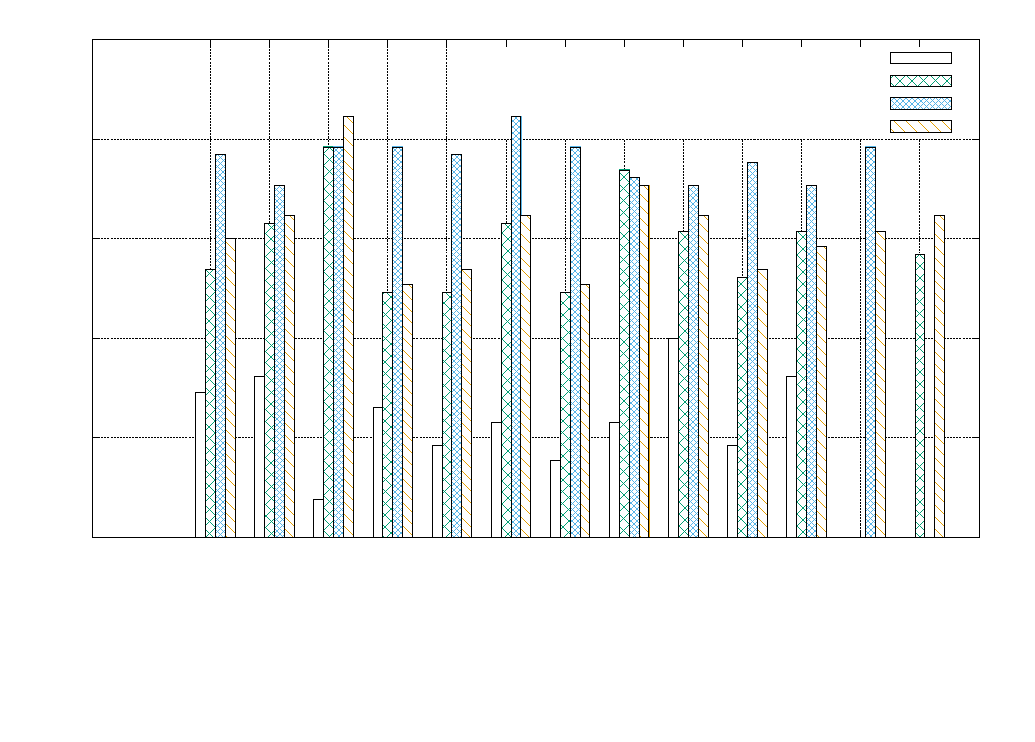
\includegraphics{myFiles/myLatex/Feature_Permutation/statereg_counter.eps}}%
    \gplfronttext
  \end{picture}%
\endgroup

            \caption{Feature Occurrence Percentage: FP State Register}
            \label{fig:Feature Occurrence Percentage: FP State Register}
        \end{figure*}
        
        \noindent
        From Figure \ref{fig:Feature Occurrence Percentage: FP Model} , similar to determining the feature importance based on the ratio shown in Figure \ref{fig:Model Accuracy Ratio ($R_n$) Per Feature}, there is no clear trend of which features are the least important across all the implementations. However, the results shown do support the observations in section \ref{subsection:determining feature importance 1},that the features "average neighbour degree" and "katz" are 2 of the more important features across all implementations. It is also worth noting that the feature "degree centrality" might be a feature that carries high importance as well. 
        
        \bigskip\noindent 
        In Figure \ref{fig:Feature Occurrence Percentage: FP State Register} the files "With fastRELIC" and "With Euclidean", has view most features to be important when predicting state registers, resulting in about $50\%$ or more for all features. These results are aligned with the results shown in \ref{fig:Model Accuracy: State Register Ratio ($SRR_n$) Per Feature} where all features are viewed to be important.
        
        \subsubsection{Conclusion for Results from Feature Permutation}
        Using feature permutation method is a way to break the correlations between features, allowing to find the most and least important features, reducing the feature set. However, from this experiment, there is a discrepancy of the features importance when comparing the data between model accuracy and state register accuracy methods. Hence a clear conclusion of which features is of least importance cannot be drawn. Further exploration is required to select features using Feature Permutation methodology.
        
        
        \newpage\subsection{Sequential Feature Selection}\label{subsection:Sequential Feature Selection result}
        Sequential Feature Selection was initially implemented after feature permutation, to further reduce the feature set and find the best combination of features. However, this resulted in less than low occurrence for almost all features. To illustrate this, method 2 of determining feature importance is used. 
        
        \begin{figure*}[ht]
        \centering
            % GNUPLOT: LaTeX picture with Postscript
\begingroup
  \makeatletter
  \providecommand\color[2][]{%
    \GenericError{(gnuplot) \space\space\space\@spaces}{%
      Package color not loaded in conjunction with
      terminal option `colourtext'%
    }{See the gnuplot documentation for explanation.%
    }{Either use 'blacktext' in gnuplot or load the package
      color.sty in LaTeX.}%
    \renewcommand\color[2][]{}%
  }%
  \providecommand\includegraphics[2][]{%
    \GenericError{(gnuplot) \space\space\space\@spaces}{%
      Package graphicx or graphics not loaded%
    }{See the gnuplot documentation for explanation.%
    }{The gnuplot epslatex terminal needs graphicx.sty or graphics.sty.}%
    \renewcommand\includegraphics[2][]{}%
  }%
  \providecommand\rotatebox[2]{#2}%
  \@ifundefined{ifGPcolor}{%
    \newif\ifGPcolor
    \GPcolortrue
  }{}%
  \@ifundefined{ifGPblacktext}{%
    \newif\ifGPblacktext
    \GPblacktexttrue
  }{}%
  % define a \g@addto@macro without @ in the name:
  \let\gplgaddtomacro\g@addto@macro
  % define empty templates for all commands taking text:
  \gdef\gplbacktext{}%
  \gdef\gplfronttext{}%
  \makeatother
  \ifGPblacktext
    % no textcolor at all
    \def\colorrgb#1{}%
    \def\colorgray#1{}%
  \else
    % gray or color?
    \ifGPcolor
      \def\colorrgb#1{\color[rgb]{#1}}%
      \def\colorgray#1{\color[gray]{#1}}%
      \expandafter\def\csname LTw\endcsname{\color{white}}%
      \expandafter\def\csname LTb\endcsname{\color{black}}%
      \expandafter\def\csname LTa\endcsname{\color{black}}%
      \expandafter\def\csname LT0\endcsname{\color[rgb]{1,0,0}}%
      \expandafter\def\csname LT1\endcsname{\color[rgb]{0,1,0}}%
      \expandafter\def\csname LT2\endcsname{\color[rgb]{0,0,1}}%
      \expandafter\def\csname LT3\endcsname{\color[rgb]{1,0,1}}%
      \expandafter\def\csname LT4\endcsname{\color[rgb]{0,1,1}}%
      \expandafter\def\csname LT5\endcsname{\color[rgb]{1,1,0}}%
      \expandafter\def\csname LT6\endcsname{\color[rgb]{0,0,0}}%
      \expandafter\def\csname LT7\endcsname{\color[rgb]{1,0.3,0}}%
      \expandafter\def\csname LT8\endcsname{\color[rgb]{0.5,0.5,0.5}}%
    \else
      % gray
      \def\colorrgb#1{\color{black}}%
      \def\colorgray#1{\color[gray]{#1}}%
      \expandafter\def\csname LTw\endcsname{\color{white}}%
      \expandafter\def\csname LTb\endcsname{\color{black}}%
      \expandafter\def\csname LTa\endcsname{\color{black}}%
      \expandafter\def\csname LT0\endcsname{\color{black}}%
      \expandafter\def\csname LT1\endcsname{\color{black}}%
      \expandafter\def\csname LT2\endcsname{\color{black}}%
      \expandafter\def\csname LT3\endcsname{\color{black}}%
      \expandafter\def\csname LT4\endcsname{\color{black}}%
      \expandafter\def\csname LT5\endcsname{\color{black}}%
      \expandafter\def\csname LT6\endcsname{\color{black}}%
      \expandafter\def\csname LT7\endcsname{\color{black}}%
      \expandafter\def\csname LT8\endcsname{\color{black}}%
    \fi
  \fi
    \setlength{\unitlength}{0.0500bp}%
    \ifx\gptboxheight\undefined%
      \newlength{\gptboxheight}%
      \newlength{\gptboxwidth}%
      \newsavebox{\gptboxtext}%
    \fi%
    \setlength{\fboxrule}{0.5pt}%
    \setlength{\fboxsep}{1pt}%
\begin{picture}(9636.00,6802.00)%
    \gplgaddtomacro\gplbacktext{%
      \csname LTb\endcsname%%
      \put(594,1803){\makebox(0,0)[r]{\strut{}$0$}}%
      \csname LTb\endcsname%%
      \put(594,2759){\makebox(0,0)[r]{\strut{}$0.2$}}%
      \csname LTb\endcsname%%
      \put(594,3714){\makebox(0,0)[r]{\strut{}$0.4$}}%
      \csname LTb\endcsname%%
      \put(594,4670){\makebox(0,0)[r]{\strut{}$0.6$}}%
      \csname LTb\endcsname%%
      \put(594,5625){\makebox(0,0)[r]{\strut{}$0.8$}}%
      \csname LTb\endcsname%%
      \put(594,6581){\makebox(0,0)[r]{\strut{}$1$}}%
      \csname LTb\endcsname%%
      \put(1861,1671){\rotatebox{30}{\makebox(0,0)[r]{\strut{}average neighbour degree}}}%
      \csname LTb\endcsname%%
      \put(2429,1671){\rotatebox{30}{\makebox(0,0)[r]{\strut{}betweenness centrality}}}%
      \csname LTb\endcsname%%
      \put(2996,1671){\rotatebox{30}{\makebox(0,0)[r]{\strut{}closeness centrality}}}%
      \csname LTb\endcsname%%
      \put(3564,1671){\rotatebox{30}{\makebox(0,0)[r]{\strut{}clustering}}}%
      \csname LTb\endcsname%%
      \put(4131,1671){\rotatebox{30}{\makebox(0,0)[r]{\strut{}degree}}}%
      \csname LTb\endcsname%%
      \put(4699,1671){\rotatebox{30}{\makebox(0,0)[r]{\strut{}degree centrality}}}%
      \csname LTb\endcsname%%
      \put(5266,1671){\rotatebox{30}{\makebox(0,0)[r]{\strut{}has feedback path}}}%
      \csname LTb\endcsname%%
      \put(5834,1671){\rotatebox{30}{\makebox(0,0)[r]{\strut{}katz}}}%
      \csname LTb\endcsname%%
      \put(6401,1671){\rotatebox{30}{\makebox(0,0)[r]{\strut{}load centrality}}}%
      \csname LTb\endcsname%%
      \put(6969,1671){\rotatebox{30}{\makebox(0,0)[r]{\strut{}outdegree}}}%
      \csname LTb\endcsname%%
      \put(7536,1671){\rotatebox{30}{\makebox(0,0)[r]{\strut{}pagerank}}}%
      \csname LTb\endcsname%%
      \put(8104,1671){\rotatebox{30}{\makebox(0,0)[r]{\strut{}euclidean}}}%
      \csname LTb\endcsname%%
      \put(8671,1671){\rotatebox{30}{\makebox(0,0)[r]{\strut{}fastRELIC}}}%
    }%
    \gplgaddtomacro\gplfronttext{%
      \csname LTb\endcsname%%
      \put(6403,6408){\makebox(0,0)[r]{\strut{}Original}}%
      \csname LTb\endcsname%%
      \put(6403,6188){\makebox(0,0)[r]{\strut{}With fastRELIC}}%
      \csname LTb\endcsname%%
      \put(6403,5968){\makebox(0,0)[r]{\strut{}With Euclidean}}%
      \csname LTb\endcsname%%
      \put(6403,5748){\makebox(0,0)[r]{\strut{}With Euclidean and fastRELIC}}%
    }%
    \gplbacktext
    \put(0,0){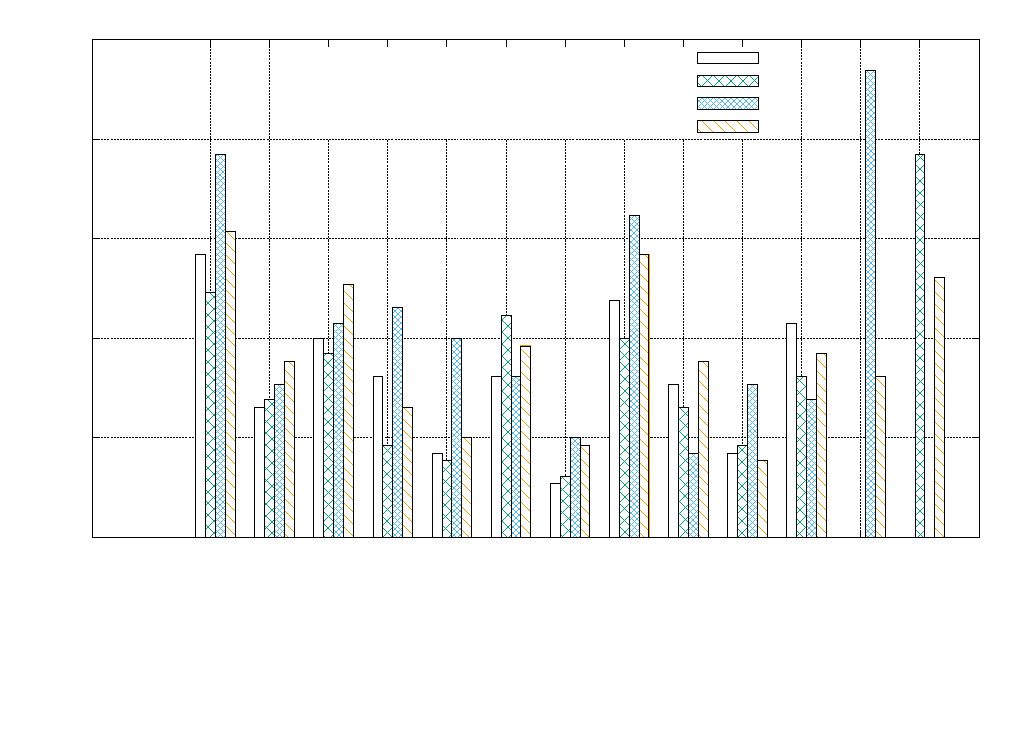
\includegraphics{./Results/Sequential_Feature_Selection/SFSafterFPComplied_count.eps}}%
    \gplfronttext
  \end{picture}%
\endgroup

            \caption{Feature Occurrence Percentage: Sequential Feature Selection after Feature Permutation}
            \label{fig:Feature Occurrence Percentage: Sequential Feature Selection after Feature Permutation}
        \end{figure*}
        
        \noindent
        As observed in Figure \ref{fig:Feature Occurrence Percentage: Sequential Feature Selection after Feature Permutation}, all but two of the primary features appears more than $50\%$ of across all implementations. Though the results support the importance of the feature "average neighbour degree" and " and katz". A test with fewer than 7 features has shown to be poor performing in the pre-optimized neural network with less than $20\%$ accuracy. Thus, SFS is used independently to support the findings of feature permutation.
        
        
        \bigskip\noindent
        To apply Step Features Selection independently, ensuring consistency, Sequential Feature Selection was repeated 5 times per file. Method 2, feature occurrence percentage is then applied to determine overall feature importance. Using the same mathematical equation in Equation \ref{eqn:percentage of feature occurrence}, the percentage of occurrence for all features across all files and runs were calculated and is presented in Figure \ref{fig:Feature Occurrence Percentage: Sequential Feature Selection}.
        
        
        \newpage\begin{figure*}
        \centering
            % GNUPLOT: LaTeX picture with Postscript
\begingroup
  \makeatletter
  \providecommand\color[2][]{%
    \GenericError{(gnuplot) \space\space\space\@spaces}{%
      Package color not loaded in conjunction with
      terminal option `colourtext'%
    }{See the gnuplot documentation for explanation.%
    }{Either use 'blacktext' in gnuplot or load the package
      color.sty in LaTeX.}%
    \renewcommand\color[2][]{}%
  }%
  \providecommand\includegraphics[2][]{%
    \GenericError{(gnuplot) \space\space\space\@spaces}{%
      Package graphicx or graphics not loaded%
    }{See the gnuplot documentation for explanation.%
    }{The gnuplot epslatex terminal needs graphicx.sty or graphics.sty.}%
    \renewcommand\includegraphics[2][]{}%
  }%
  \providecommand\rotatebox[2]{#2}%
  \@ifundefined{ifGPcolor}{%
    \newif\ifGPcolor
    \GPcolortrue
  }{}%
  \@ifundefined{ifGPblacktext}{%
    \newif\ifGPblacktext
    \GPblacktexttrue
  }{}%
  % define a \g@addto@macro without @ in the name:
  \let\gplgaddtomacro\g@addto@macro
  % define empty templates for all commands taking text:
  \gdef\gplbacktext{}%
  \gdef\gplfronttext{}%
  \makeatother
  \ifGPblacktext
    % no textcolor at all
    \def\colorrgb#1{}%
    \def\colorgray#1{}%
  \else
    % gray or color?
    \ifGPcolor
      \def\colorrgb#1{\color[rgb]{#1}}%
      \def\colorgray#1{\color[gray]{#1}}%
      \expandafter\def\csname LTw\endcsname{\color{white}}%
      \expandafter\def\csname LTb\endcsname{\color{black}}%
      \expandafter\def\csname LTa\endcsname{\color{black}}%
      \expandafter\def\csname LT0\endcsname{\color[rgb]{1,0,0}}%
      \expandafter\def\csname LT1\endcsname{\color[rgb]{0,1,0}}%
      \expandafter\def\csname LT2\endcsname{\color[rgb]{0,0,1}}%
      \expandafter\def\csname LT3\endcsname{\color[rgb]{1,0,1}}%
      \expandafter\def\csname LT4\endcsname{\color[rgb]{0,1,1}}%
      \expandafter\def\csname LT5\endcsname{\color[rgb]{1,1,0}}%
      \expandafter\def\csname LT6\endcsname{\color[rgb]{0,0,0}}%
      \expandafter\def\csname LT7\endcsname{\color[rgb]{1,0.3,0}}%
      \expandafter\def\csname LT8\endcsname{\color[rgb]{0.5,0.5,0.5}}%
    \else
      % gray
      \def\colorrgb#1{\color{black}}%
      \def\colorgray#1{\color[gray]{#1}}%
      \expandafter\def\csname LTw\endcsname{\color{white}}%
      \expandafter\def\csname LTb\endcsname{\color{black}}%
      \expandafter\def\csname LTa\endcsname{\color{black}}%
      \expandafter\def\csname LT0\endcsname{\color{black}}%
      \expandafter\def\csname LT1\endcsname{\color{black}}%
      \expandafter\def\csname LT2\endcsname{\color{black}}%
      \expandafter\def\csname LT3\endcsname{\color{black}}%
      \expandafter\def\csname LT4\endcsname{\color{black}}%
      \expandafter\def\csname LT5\endcsname{\color{black}}%
      \expandafter\def\csname LT6\endcsname{\color{black}}%
      \expandafter\def\csname LT7\endcsname{\color{black}}%
      \expandafter\def\csname LT8\endcsname{\color{black}}%
    \fi
  \fi
    \setlength{\unitlength}{0.0500bp}%
    \ifx\gptboxheight\undefined%
      \newlength{\gptboxheight}%
      \newlength{\gptboxwidth}%
      \newsavebox{\gptboxtext}%
    \fi%
    \setlength{\fboxrule}{0.5pt}%
    \setlength{\fboxsep}{1pt}%
\begin{picture}(9636.00,6802.00)%
    \gplgaddtomacro\gplbacktext{%
      \csname LTb\endcsname%%
      \put(594,1803){\makebox(0,0)[r]{\strut{}$0.2$}}%
      \csname LTb\endcsname%%
      \put(594,2759){\makebox(0,0)[r]{\strut{}$0.4$}}%
      \csname LTb\endcsname%%
      \put(594,3714){\makebox(0,0)[r]{\strut{}$0.6$}}%
      \csname LTb\endcsname%%
      \put(594,4670){\makebox(0,0)[r]{\strut{}$0.8$}}%
      \csname LTb\endcsname%%
      \put(594,5625){\makebox(0,0)[r]{\strut{}$1$}}%
      \csname LTb\endcsname%%
      \put(594,6581){\makebox(0,0)[r]{\strut{}$1.2$}}%
      \csname LTb\endcsname%%
      \put(1861,1671){\rotatebox{30}{\makebox(0,0)[r]{\strut{}average neighbour degree}}}%
      \csname LTb\endcsname%%
      \put(2429,1671){\rotatebox{30}{\makebox(0,0)[r]{\strut{}betweenness centrality}}}%
      \csname LTb\endcsname%%
      \put(2996,1671){\rotatebox{30}{\makebox(0,0)[r]{\strut{}closeness centrality}}}%
      \csname LTb\endcsname%%
      \put(3564,1671){\rotatebox{30}{\makebox(0,0)[r]{\strut{}clustering}}}%
      \csname LTb\endcsname%%
      \put(4131,1671){\rotatebox{30}{\makebox(0,0)[r]{\strut{}degree}}}%
      \csname LTb\endcsname%%
      \put(4699,1671){\rotatebox{30}{\makebox(0,0)[r]{\strut{}degree centrality}}}%
      \csname LTb\endcsname%%
      \put(5266,1671){\rotatebox{30}{\makebox(0,0)[r]{\strut{}has feedback path}}}%
      \csname LTb\endcsname%%
      \put(5834,1671){\rotatebox{30}{\makebox(0,0)[r]{\strut{}katz}}}%
      \csname LTb\endcsname%%
      \put(6401,1671){\rotatebox{30}{\makebox(0,0)[r]{\strut{}load centrality}}}%
      \csname LTb\endcsname%%
      \put(6969,1671){\rotatebox{30}{\makebox(0,0)[r]{\strut{}outdegree}}}%
      \csname LTb\endcsname%%
      \put(7536,1671){\rotatebox{30}{\makebox(0,0)[r]{\strut{}pagerank}}}%
      \csname LTb\endcsname%%
      \put(8104,1671){\rotatebox{30}{\makebox(0,0)[r]{\strut{}euclidean}}}%
      \csname LTb\endcsname%%
      \put(8671,1671){\rotatebox{30}{\makebox(0,0)[r]{\strut{}fastRELIC}}}%
    }%
    \gplgaddtomacro\gplfronttext{%
      \csname LTb\endcsname%%
      \put(8252,6408){\makebox(0,0)[r]{\strut{}Original}}%
      \csname LTb\endcsname%%
      \put(8252,6188){\makebox(0,0)[r]{\strut{}With fastRELIC}}%
      \csname LTb\endcsname%%
      \put(8252,5968){\makebox(0,0)[r]{\strut{}With Euclidean}}%
      \csname LTb\endcsname%%
      \put(8252,5748){\makebox(0,0)[r]{\strut{}With Euclidean and fastRELIC}}%
    }%
    \gplbacktext
    \put(0,0){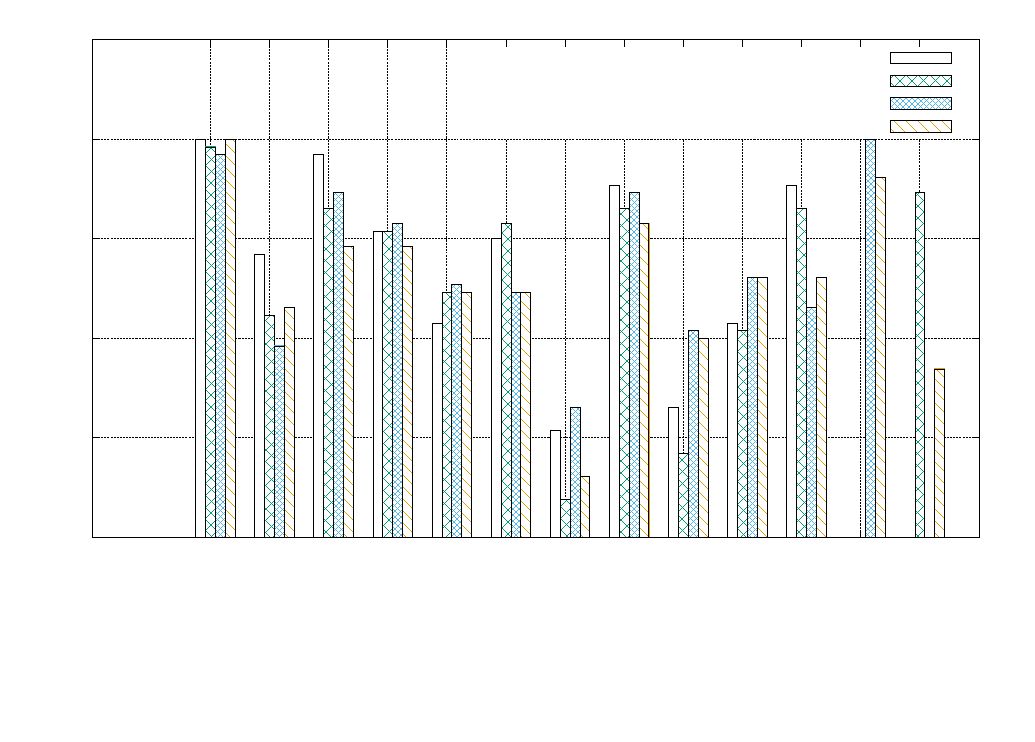
\includegraphics{SFS}}%
    \gplfronttext
  \end{picture}%
\endgroup

            \caption{Feature Occurrence Percentage: Sequential Feature Selection}
            \label{fig:Feature Occurrence Percentage: Sequential Feature Selection}
        \end{figure*}
        
        \bigskip\noindent
        From Figure \ref{fig:Feature Occurrence Percentage: Sequential Feature Selection} there is support for the observations to the feature permutation methodology, which is the 2 most important primary features are "average neighbour degree" and "katz". Additionally, from Figure \ref{fig:Feature Occurrence Percentage: Sequential Feature Selection}, across all implementations, the feature "has feedback path" does not appear more than $50\%$ for all 5 runs. To test the importance of features occurring less than $50\%$ for all 5 runs, those features are removed in all implementations respectively and re-tested for another 5 times.
        
        \bigskip\noindent
        From Table \ref{tab:Model Accuracy after Step Feature Selection} and \ref{tab:State Register Accuracy after Step Feature Selection}, the average of 5 run are almost identical to Table \ref{tab:Model Accuracy No Feature Selection} and \ref{tab:State Register Accuracy No Feature Selection}, with only a difference in less than $2\%$. This suggests that the respective removed feature(s), does not add any value to the machine learning process. Removing these feature(s) will therefore decrease the computation time required for the neural network. However, since the feature(s) removed were not the same for all implementation, based on Table \ref{tab:Model Accuracy after Step Feature Selection} and \ref{tab:State Register Accuracy after Step Feature Selection}, the conclusion that both "has feedback path" and "load centrality" features does not add any value to the neural network for all implementation cannot be drawn.
        
       \bigskip\noindent
        To confirm that both features do not add value to the neural network regardless of implementation for additional features, the same amount of features will have to be removed across all implementations and the process will have to be repeated. Previously, the files "With Euclidean" and the files "With Euclidean and fastRELIC", only had the feature "had feedback path" removed. Repeating the process for only these 2 implementation removing both the feature "has feedback path" and "load centrality", yields the results shown in Table \ref{tab:Model Accuracy Feature Redundant} and \ref{tab:State Register Accuracy Feature Redundant}. 
        
        \begin{table}
            \centering
            \begin{tabular}{|c|c|c|c|c|}
    \hline
     & \multicolumn{4}{c|}{Model Accuracy}\\
    \cline {2-5}
    File Name & Original & With fastRELIC & With Euclidean & With Euclidean and fastRELIC\\
    \hline
    \hline
    b01\_reset.csv & 0.97 & 0.97 & 0.98 & 0.96\\
    \hline
    b02\_reset.csv & 0.91 & 0.94 & 0.94 & 0.90\\
    \hline
    b04\_reset.csv & 0.57 & 0.81 & 0.98 & 0.99\\
    \hline
    b06\_reset.csv & 1.00 & 1.00 & 1.00 & 1.00\\
    \hline
    b08\_reset.csv & 0.57 & 0.91 & 0.84 & 0.91\\
    \hline
    b09\_reset.csv & 0.63 & 0.79 & 0.65 & 0.73\\
    \hline
    b10\_reset.csv & 0.73 & 0.81 & 0.76 & 0.83\\
    \hline
    b14\_reset.csv & 0.56 & 0.68 & 0.61 & 0.66\\
    \hline
    completogpio.csv & 0.84 & 0.88 & 0.86 & 0.87\\
    \hline
    FSM.csv & 0.65 & 0.79 & 0.71 & 0.80\\
    \hline
    MEMORY\_INTERFACE.csv & 0.93 & 0.97 & 0.96 & 0.97\\
    \hline
    spi\_axi\_master.csv & 0.98 & 0.98 & 0.96 & 0.91\\
    \hline
    uart.csv & 0.44 & 0.72 & 0.55 & 0.70\\
    \hline
    \hline
    average & 0.75 & 0.86 & 0.83 & 0.86\\
    \hline
\end{tabular}
\caption{Model Accuracy}
\label{tab:Model Accuracy after Step Feature Selection}


        \end{table}      
        
        \begin{table}
            \centering
            \bigskip\begin{tabular}{|c|c|c|c|c|}
    \hline
     & \multicolumn{4}{c|}{State Register Accuracy}\\
    \cline {2-5}
    File Name & Original & With fastRELIC & With Euclidean & With Euclidean and fastRELIC\\
    \hline
    \hline
    b01\_reset.csv & 0.95 & 0.95 & 0.97 & 0.94\\
    \hline
    b02\_reset.csv & 0.88 & 0.92 & 0.91 & 0.87\\
    \hline
    b04\_reset.csv & 0.36 & 0.89 & 0.53 & 0.82\\
    \hline
    b06\_reset.csv & 0.99 & 1.00 & 0.99 & 1.00\\
    \hline
    b08\_reset.csv & 0.45 & 0.62 & 0.32 & 0.64\\
    \hline
    b09\_reset.csv & 0.86 & 0.95 & 0.97 & 0.96\\
    \hline
    b10\_reset.csv & 0.87 & 0.88 & 0.93 & 0.90\\
    \hline
    b14\_reset.csv & 0.59 & 0.21 & 0.28 & 0.22\\
    \hline
    completogpio.csv & 0.49 & 0.98 & 1.00 & 1.00\\
    \hline
    FSM.csv & 0.40 & 0.79 & 0.56 & 0.84\\
    \hline
    MEMORY\_INTERFACE.csv & 0.30 & 0.63 & 0.54 & 0.63\\
    \hline
    spi\_axi\_master.csv & 0.32 & 0.50 & 0.71 & 0.68\\
    \hline
    uart.csv & 0.24 & 0.75 & 0.45 & 0.68\\
    \hline
    \hline
    average & 0.59 & 0.77 & 0.70 & 0.78\\
    \hline
\end{tabular}
\caption{State Register Accuracy}
\label{tab:State Register Accuracy after Step Feature Selection}

        \end{table}
        
        \begin{table}
            \centering
            \begin{tabular}{|c|c|c|}
    \hline
     & \multicolumn{2}{c|}{Model Accuracy}\\
    \cline {2-3}
    File Name & With Euclidean & With Euclidean and fastRELIC \\
    \hline
    \hline
    b01\_reset.csv & 0.99 & 0.97\\
    \hline
    b02\_reset.csv & 0.91 & 0.86\\
    \hline
    b04\_reset.csv & 0.98 & 0.99\\
    \hline
    b06\_reset.csv & 1.00 & 1.00\\
    \hline
    b08\_reset.csv & 0.82 & 0.91\\
    \hline
    b09\_reset.csv & 0.66 & 0.79\\
    \hline
    b10\_reset.csv & 0.79 & 0.85\\
    \hline
    b14\_reset.csv & 0.61 & 0.66\\
    \hline
    completogpio.csv & 0.86 & 0.87\\
    \hline
    FSM.csv & 0.71 & 0.80\\
    \hline
    MEMORY\_INTERFACE.csv & 0.96 & 0.96\\
    \hline
    spi\_axi\_master.csv & 0.96 &0.92\\
    \hline
    uart.csv & 0.53 & 0.69\\
    \hline
    \hline
    average & 0.83 & 0.87\\
    \hline
\end{tabular}
\caption{Model Accuracy}
\label{tab:Model Accuracy Feature Redundant}

        \end{table}
        
        \begin{table}
            \centering
            \bigskip\begin{tabular}{|c|c|c|}
    \hline
     & \multicolumn{2}{c|}{State Register Accuracy}\\
    \cline {2-3}
    File Name & With Euclidean & With Euclidean and fastRELIC \\
    \hline
    \hline
    completogpio.csv & 0.98 & 0.95\\
    \hline
    b02\_reset.csv & 0.88 & 0.82\\
    \hline
    b04\_reset.csv & 0.55 & 0.81\\
    \hline
    b06\_reset.csv & 0.99 & 1.00\\
    \hline
    b08\_reset.csv & 0.27 & 0.63\\
    \hline
    b09\_reset.csv & 0.99 & 0.95\\
    \hline
    b10\_reset.csv & 0.95 & 0.89\\
    \hline
    b14\_reset.csv & 0.26 & 0.18\\
    \hline
    completogpio.csv & 1.00 & 1.00\\
    \hline
    FSM.csv & 0.56 & 0.88\\
    \hline
    MEMORY\_INTERFACE.csv & 0.53 & 0.62\\
    \hline
    spi\_axi\_master.csv & 0.71 & 0.67\\
    \hline
    uart.csv & 0.43 & 0.67\\
    \hline
    \hline
    average & 0.70 & 0.77\\
    \hline
\end{tabular}
\caption{State Register Accuracy}
\label{tab:State Register Accuracy Feature Redundant}
        \end{table}
        
        
        \newpage\subsubsection{Conclusion for Sequential Feature Selection}
        Sequential Feature Selection has supported the observations from Feature Permutation, as well as gave insights to which Features are a hindrance/redundant. From Table \ref{tab:Model Accuracy Feature Redundant} and \ref{tab:State Register Accuracy Feature Redundant}, both the Model Accuracy and State Register Accuracy was minimally affected, even when both features "has feedback path" and "load centrality" have been removed. To further improve this results, further test with more features removed, using a higher threshold for percentage of feature
        selection can be used.  
    
        \subsection{Implementation Selection}
        Based on the results obtained, the two best performing implementations are "With fastRELIC" and "With Euclidean and fastRELIC". As the implementation "With fastRELIC" has performed similarly well when compared to the implementation "With Euclidean and fastRELIC" with a feature lesser, the implementation "With fastRELIC" will be chosen for hyperparameter tuning.  
    
    \newpage\section{Talos Hyperparameter Tuning}\label{Talos Tunning}
    Briefly mentioned in section \ref{subsection:implementing additional features} was a method to optimize the neural network. The "Talos" module is used to automate the repeated training and testing process of the neural network, with a range of preset parameters. The most optimized model is determined by "Talos" based on a set metric. The model can then be deployed for predictions or further training. 
    
    
    \bigskip\noindent
    The range of hyperparameters that is automated with "Talos" is shown in table \ref{tab:Final Talos Parameters}:
    
            \begin{table}[ht]
            \centering
            \begin{tabular}{|c|c|}
    \hline
    Hyperparameter & Input\\
    \hline
    \hline
    Optimizer & Adam, RMSprop  \\
    \hline
    Loss Function & Binary Crossentropy, Sparse Categorical Crossentropy  \\
    \hline
    Batch Size & 10, 32\\
    \hline
    Epochs & 1, 5, 10, 24\\
    \hline
    Dropout & 0, 0.25, 0.5 \\
    \hline
    First Neurons & 20, to 80, increment of 4 per step  \\
    \hline
    Hidden Layers & 5, 15, 35  \\
    \hline
    Hidden Neurons & 7 to 490, increment of 7 per step  \\
    \hline
    Hidden Layer Activation Function & ReLU, ELU\\
    \hline
    Last Activation Function & Sigmoid\\
    \hline
\end{tabular}
\caption{Talos Parameters}
\label{tab:Final Talos Parameters}
            \end{table}
            
            
    \section{Tuning Model 1}\label{section:tuning b14}
    The file used for testing has been selected to be "b14\_reset.csv". This is due to the file containing near 20\% of all registers. By default, "Talos" uses grid search to process and find the most optimal hyperparameter however, due to the large number of permutations, high number of hidden layers and hidden neurons, using grid search resulted in a really slow process. Therefore, random search of 20\% of the permutations with a probabilistic reduction using the metric "forest" was used to find the most optimal hyperparameters. Two of the hyperparameter permutation which resulted in the highest accuracy was then chosen shown in \ref{tab:Optimal Hyperparameters b14}, represented as Model 1 and Model 2 .
        
    \bigskip\noindent
    From the hyperparameter tuning, the optimal hyperparameters from Talos is shown in table \ref{tab:Optimal Hyperparameters b14}
    
        \begin{table}[ht]
            \centering
            \begin{tabular}{|c|c|c|}
    \hline
    Hyperparameter & Model 1 & Model 2\\
    \hline
    \hline
    Optimizer & adam &  adam \\
    \hline
    Loss Function & Sparse Categorical Crossentropy &  Binary Crossentropy \\
    \hline
    Batch Size & 32 & 32\\
    \hline
    Epochs & 1 & 10\\
    \hline
    Dropout & 0.25 & 0 \\
    \hline
    First Neurons & 35 & 50\\
    \hline
    Hidden Layers & 5 & 35\\
    \hline
    Hidden Neurons & 7 & 287\\
    \hline
    Hidden Layer Activation Function & ReLU & ReLu\\
    \hline
    Last Activation Function & Sigmoid & Sigmoid\\
    \hline
\end{tabular}
\caption{Optimal Hyperparameters (b14\_reset)}
\label{tab:Optimal Hyperparameters b14}
        \end{table}
    
    \newpage\subsubsection{Deploying Model 1}
    Recreating these 2 models, the models were evaluated for accuracy and state register accuracy for a total of 500 times per file and the average accuracy across all files was then calculated. The results are shown in Table \ref{tab:Optimized Model Accuracy (b14)}.
            
        \begin{table}[ht]
            \centering
            \bigskip\begin{tabular}{|c|c|c|c|c|}
    \hline
     & \multicolumn{2}{c|}{Model Accuracy} & \multicolumn{2}{c|}{State Register Accuracy}\\
    \cline {2-5}
    File Name & Model 1 & Model 2 & Model 1 & Model 2 \\
    \hline
    \hline
    b01\_reset.csv & 0.71 & 0.62 & 0.54 & 0.38\\
    \hline
    b02\_reset.csv & 0.63 & 0.54 & 0.53 & 0.40\\
    \hline
    b04\_reset.csv & 0.95 & 0.92 & 0.44 & 0.43\\
    \hline
    b06\_reset.csv & 0.80 & 0.76 & 0.59 & 0.43\\
    \hline
    b08\_reset.csv & 0.83 & 0.81 & 0.39 & 0.27\\
    \hline
    b09\_reset.csv & 0.81 & 0.84 & 0.63 & 0.43\\
    \hline
    b10\_reset.csv & 0.78 & 0.77 & 0.62 & 0.39\\
    \hline
    b14\_reset.csv & 0.84 & 0.82 & 0.66 & 0.48\\
    \hline
    completogpio.csv & 0.87 & 0.83 & 0.45 & 0.36\\
    \hline
    FSM.csv & 0.68 & 0.63 & 0.49 & 0.35\\
    \hline
    MEMORY\_INTERFACE.csv & 0.92 & 0.93 & 0.15 & 0.24\\
    \hline
    spi\_axi\_master.csv & 0.98 & 0.96 & 0.04 & 0.32\\
    \hline
    uart.csv & 0.27 & 0.33 & 0.01 & 0.11\\
    \hline
    \hline
    average & 0.77 & 0.75 & 0.43 & 0.35\\
\hline
\end{tabular}
\caption{Optimized Model Accuracy (b14\_reset)}
\label{tab:Optimized Model Accuracy (b14)}
        \end{table}
        
        \noindent
        From Table \ref{tab:Optimized Model Accuracy (b14)} the accuracy was high, yet the state register accuracy remains very low for both models. From these results, it can be observed that this model performed worse than the pre-optimized neural network. The following conclusions can therefore be drawn:
        
        \begin{itemize}
            \item Model resulted in high false negative rate
            \item b14\_reset.csv is not suitable for testing due to the low amount of state registers in the file and due to the file containing valuable information for training.
            \item There is no or low correlation between Model Accuracy and State Register Accuracy 
        \end{itemize}
        
    
    \newpage\section{Tuning Model 2}\label{section:tuning uart}
    Due to the poor results produced in section \ref{section:tuning b14} the tuning process was repeated using "uart.csv" instead. "uart.csv", though it contains less registers, it has an even spread of state register and non-state registers. This makes it ideal for testing the neural network during the tuning process. Similarly, 2 best performing hyperparameter permutations were recreated and tested for 500 times.
    
        \begin{table}[ht]
            \centering
            \begin{tabular}{|c|c|c|}
    \hline
    Hyperparameter & Model 1 & Model 2\\
    \hline
    \hline
    Optimizer & adam &  RMSprop \\
    \hline
    Loss Function & Sparse Categorical Crossentropy &  Binary Crossentropy \\
    \hline
    Batch Size & 32 & 10\\
    \hline
    Epochs & 5 & 10\\
    \hline
    Dropout & 0 & 0.5 \\
    \hline
    First Neurons & 20 & 20\\
    \hline
    Hidden Layers & 15 & 15\\
    \hline
    Hidden Neurons & 7 & 217\\
    \hline
    Hidden Layer Activation Function & ReLU & ELU\\
    \hline
    Last Activation Function & Sigmoid & Sigmoid\\
    \hline
\end{tabular}
\caption{Optimal Hyperparameters (uart)}
\label{tab:Optimal Hyperparameters uart}
        \end{table}
    
    \subsubsection{Deploying Model 2}
    The results are shown in table 
    
        \begin{table}[ht]
            \centering
            \bigskip\begin{tabular}{|c|c|c|c|c|}
    \hline
     & \multicolumn{2}{c|}{Model Accuracy} & \multicolumn{2}{c|}{State Register Accuracy}\\
    \cline {2-5}
    File Name & Model 1 & Model 2 & Model 1 & Model 2\\
    \hline
    \hline
    b01\_reset.csv & 0.41 & 0.80 & 0.02 & 0.98\\
    \hline
    b02\_reset.csv & 0.28 & 0.86 & 0.04 & 0.98\\
    \hline
    b04\_reset.csv & 0.97 & 0.66 & 0.02 & 0.96\\
    \hline
    b06\_reset.csv & 0.63 & 0.55 & 0.04 & 0.99\\
    \hline
    b08\_reset.csv & 0.77 & 0.44 & 0.03 & 0.98\\
    \hline
    b09\_reset.csv & 0.92 & 0.36 & 0.04 & 0.99\\
    \hline
    b10\_reset.csv & 0.77 & 0.55 & 0.03 & 0.99\\
    \hline
    b14\_reset.csv & 0.99 & 0.56 & 0.05 & 0.99\\
    \hline
    completogpio.csv & 0.79 & 0.66 & 0.01 & 0.97\\
    \hline
    FSM.csv & 0.54 & 0.55 & 0.02 & 0.99\\
    \hline
    MEMORY\_INTERFACE.csv & 0.91 & 0.97 & 0.00 & 0.69\\
    \hline
    spi\_axi\_master.csv & 0.99 & 0.87 & 0.00 & 0.65\\
    \hline
    uart.csv & 0.27 & 0.63 & 0.00 & 0.60\\
    \hline
    \hline
    average & 0.71 & 0.65 & 0.02 & 0.91\\
    \hline
\end{tabular}
\caption{Optimized Model Accuracy (uart)}
\label{tab:Optimized Model Accuracy (uart)}
        \end{table}
    
    
        \newpage\noindent
        It can be seen from Table \ref{tab:Optimized Model Accuracy (uart)} that though Model 1 has significantly higher model accuracy compared to Model 2, the state register accuracy is significantly lower. This suggests that Model 1 produces a significant amount of false negative, while Model 2 has a lower Model Accuracy, but significantly higher State Register Accuracy, out performing the pre-optimized model in most of the files. This suggests that Model 2 might be underfitted due to low model accuracy, thus producing a high amount of false positive.
        
        \bigskip\noindent
        To improve this result, the amount of epoch is raised from 10 to 22 shown in Table \ref{tab: Modified Optimal Hyperparameters uart}, with other hyperparameters kept the same. 
        
        \begin{table}[ht]
            \centering
            \begin{tabular}{|c|c|}
    \hline
    Hyperparameter & Model 2\\
    \hline
    \hline
    Optimizer & RMSprop\\
    \hline
    Loss Function & Binary Crossentropy\\
    \hline
    Batch Size & 10\\
    \hline
    Epochs & 22\\
    \hline
    Dropout & 0.5\\
    \hline
    First Neurons & 20\\
    \hline
    Hidden Layers & 15\\
    \hline
    Hidden Neurons & 217\\
    \hline
    Hidden Layer Activation Function & ELU\\
    \hline
    Last Activation Function & Sigmoid\\
    \hline
\end{tabular}
\caption{Modified Optimal Hyperparameters (uart)}
\label{tab: Modified Optimal Hyperparameters uart}
        \end{table}
        
        The results is shown in table \ref{tab:Modified Optimized Model Accuracy (uart)}
        
        \begin{table}[ht]
            \centering
            \bigskip\begin{tabular}{|c|c|c|}
    \hline
    File Name & Model Accuracy & State Register Accuracy\\
    \hline
    \hline
    b01\_reset.csv & 0.95 & 0.99\\
    \hline
    b02\_reset.csv & 0.93 & 0.99\\
    \hline
    b04\_reset.csv & 0.69 & 0.94\\
    \hline
    b06\_reset.csv & 0.83 & 1.00\\
    \hline
    b08\_reset.csv & 0.73 & 0.97\\
    \hline
    b09\_reset.csv & 0.56 & 0.99\\
    \hline
    b10\_reset.csv & 0.67 & 1.00\\
    \hline
    b14\_reset.csv & 0.53 & 1.00\\
    \hline
    completogpio.csv & 0.81 & 0.96\\
    \hline
    FSM.csv & 0.64 & 0.98\\
    \hline
    MEMORY\_INTERFACE.csv & 0.99 & 0.85\\
    \hline
    spi\_axi\_master.csv & 0.85 & 0.66\\
    \hline
    uart.csv & 0.56 & 0.48\\
    \hline
    \hline
    average & 0.75 & 0.91\\
    \hline
\end{tabular}
\caption{Modified Optimized Model Accuracy (uart)}
\label{tab:Modified Optimized Model Accuracy (uart)}
        \end{table}
        
    \newpage\section{Conclusion for Tuning Neural Network}
    By increasing the epoch from 10 to 22 shown in \ref{tab:Modified Optimized Model Accuracy (uart)}, the average model accuracy has increased by a significant $10\%$, while keeping the average State Register Accuracy the same. This increment implies a significantly lesser false positive on average compared to the original optimal hyperparameters shown in \ref{tab:Optimized Model Accuracy (uart)} (Model 2).
    
    \bigskip\noindent
    With an overall increase per file in Model Accuracy, it is worth noting that not all per file Model Accuracy is high even if there is an overall increase. This is especially true when observing the results in Table \ref{tab:Modified Optimized Model Accuracy (uart)} for the file "uart.csv". "uart.csv" is the worst performing file with a significant decrease in both Model Accuracy and State Register Accuracy after changing the epoch, thus showing this neural network can still be further optimized.
    
    \bigskip\noindent
    Comparing the implementation "With fastRELIC" results of the tuned model in Table \ref{tab:Modified Optimized Model Accuracy (uart)} to the results of the pre-optimize model in Table \ref{tab:Model Accuracy after Step Feature Selection} and Table \ref{tab:State Register Accuracy after Step Feature Selection}, the Model Accuracy has decrease, while the State Register Accuracy has increased. Though it is preferred to have both accuracy being equivalently high, there is always a trade off between these 2 metrics. However, the Model chosen should be able to produce results with a higher State Register Accuracy. A low State Register Accuracy will result in FSM extraction process impossible, while a low State Model Accuracy will result in extraction of FSM process being more difficult.

    \bigskip\noindent
    To conclude, even though the model presents a high average Model Accuracy and high average State Register Accuracy, the model does not produce a consistently high Model Accuracy and State Register Accuracy on a per file per run basis. However, with such a high accuracy on average for both metrics, this proves that Machine Learning is well suited for this application, given the  right features.
    

\chapter{Conclusion and Future Work}
    \section{Future Work}\label{section:Future Work}
    \subsection{The Data}
    A larger data set can be trial with, ensuring a good spread of State and Non-State Registers in both training and testing files.

    \subsection{Pre-Processing: Feature Selection}
    Based on the results produced, the correlation between each feature can be further looked into, filtering out even more features that will hinder the neural network. Heat maps can be used and the effects of removing highly correlated features should be studied. 
    
    \bigskip\noindent
    Though computationally more expensive, exhaustive feature selection can be tested out instead of sequential feature selection.
    
    \bigskip\noindent
    The counting algorithm used to implement fastRELIC as an additional feature, results in high performance in this experiment. However, the scores are inconsistent as the count is normalized per file. Therefore the fastRELIC result has a high dependency on the amount of registers in a file. Thus using Machine Learning to assign similarity scores to replace the reliance on fastRELIC can be explored. These 2 machine learning models can then be integrated, simplifying the entire process. 
    
    
    \subsection{Neural Network Architecture and Tuning}
    Multiple different types of neural network architecture can be tested out, with varying neurons and activation functions per layer. Instead of compiling all the training data to 1 file which is then used to train the neural network, training the neural network progressively can also be tested out with differing hyperparameters per training file. 
    
    
    \section{Conclusion}
    Comparing the results discussed in Chapter \ref{chapter:results} to the results obtained solely by the method of fastRELIC, the results of this thesis shows that State Register identification using machine learning is a viable alternative which compliments the fastRELIC method, achieving an average high Model Accuracy and State Register Accuracy. This thesis should therefore be viewed as an evolution to the fastRELIC method. However, due to the experiments only being trial on a limited data set, which achieved inconsistent results on a single run, the model must still be regarded to be in its infancy and not ready to be deployed for use. Therefore, to be able to use the model for State Register identification in the near future, further exploration discussed in Section \ref{section:Future Work} has to be explored to ensure the reliability of the model. 
    
      

\appendix

\chapter{Supplementary material}

\backmatter

\bibliographystyle{IEEEtran}
\bibliography{literature}

\end{document}



